\chapter{Design} \label{chap:design}

%\version{v1.10.2015}

\section*{}
\section{System Architecture}
  
\subsection{High Level Context Diagram}
\begin{figure}[ht]
\center
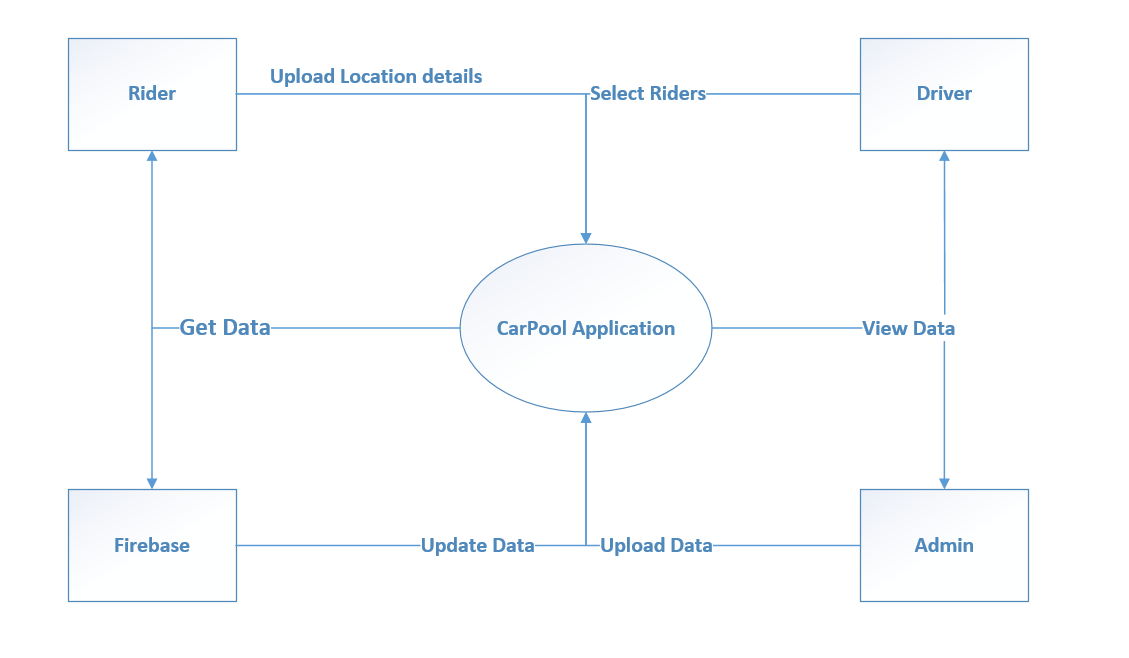
\includegraphics[width=1.2\textwidth]{SystemArchitecture}
\caption{Context Diagram}
\label{fig:Context Diagram}
\end{figure}
\begin{figure}[ht]
\center
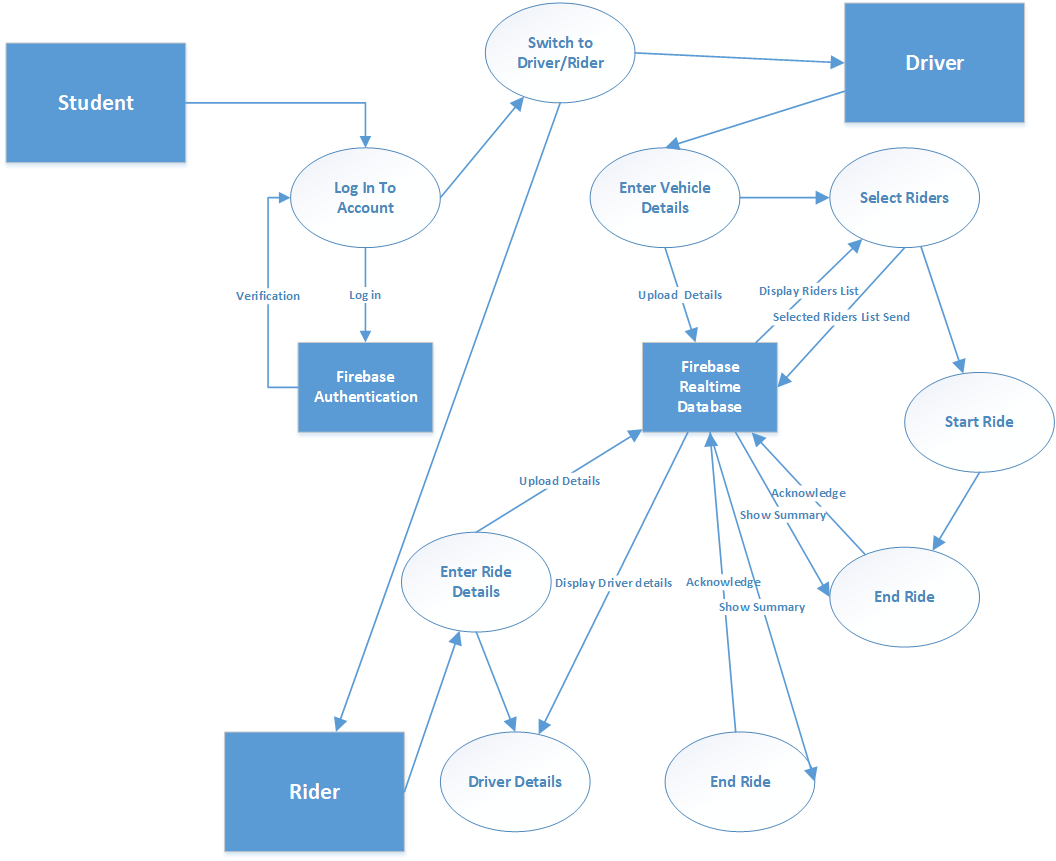
\includegraphics[width=1.2\textwidth]{SubSystem}
\caption{Sub System}
\label{fig:SubSystem}
\end{figure}

\section{Design Constraints} 
In our application we add a list of pick up points for the ease of drivers. This is made easier when clients can select pick up points and drivers reach the destination without hassle. Due to the COVID-19 pandemic, we could not be supervised and guided properly. Hence this process was not added and executed.
\section{Design Methodology}
The design of a project is important for the structure of the application by using UML (Unified Modeling Language) which is a general purpose modelling language, that aims to define a standard way to visualize the way a system has been designed. It is quite similar to blueprints used in other fields of engineering.
\\ \textbf{Reasons to use UML for project analysis and design are:} 

\begin{itemize}
\item Complex applications need collaboration and planning from multiple teams and hence require a clear and concise way to communicate amongst them.
\item A lot of time is saved down the line when teams are able to visualize processes, user interactions and static structure of the system.
These project designs will try and make the overall idea of the project more
understandable and clear by identifying Actors and functional / non-functional needs,
And also all the diagrams needed to give a clear view about this project.

\end{itemize}
\section{High-Level Design}
\subsection{Conceptual or Logical: UML Package diagram} 

\begin{figure}[ht]
\center
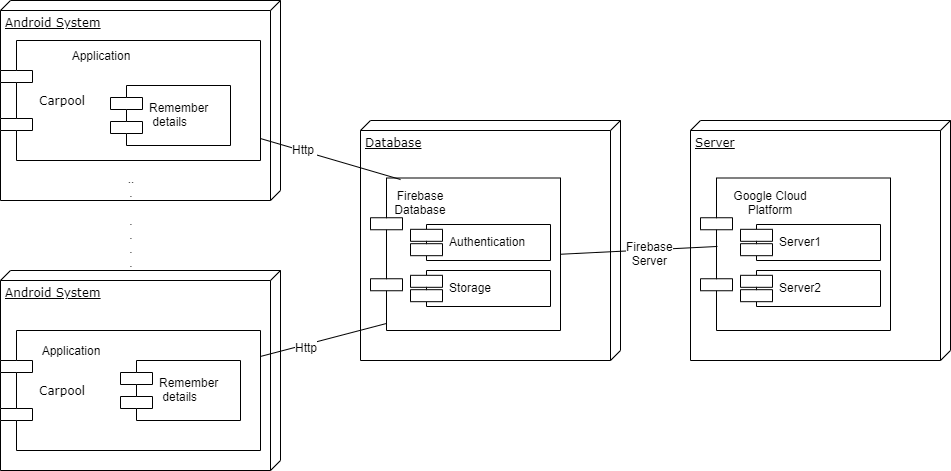
\includegraphics[width=1.0\textwidth]{PackageDiagram}
\caption{Package Diagram}
\label{fig:Package Diagram}
\end{figure}
\clearpage
\begin{figure}
\subsection{Process Interaction Diagram}
\center
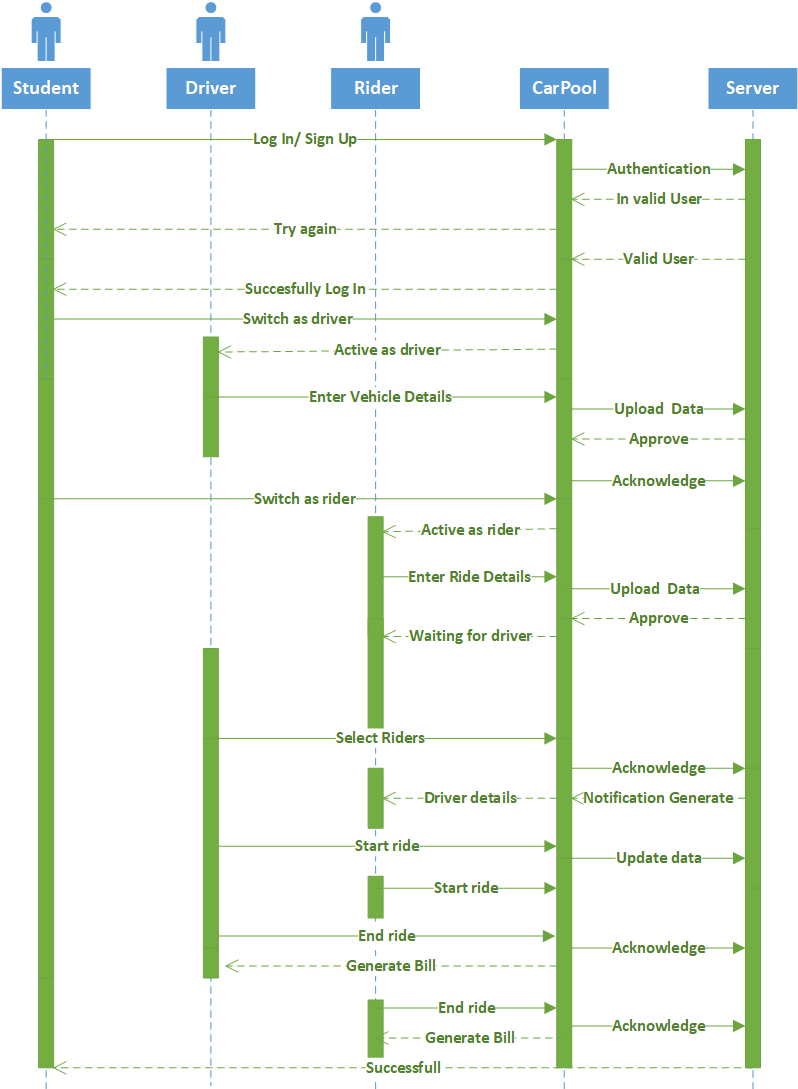
\includegraphics[width=15cm,height=25cm,keepaspectratio]{InteractionDiagram}
\caption{Process Interaction Diagram}
\label{fig:Process Interaction Diagram}
\end{figure}

\begin{figure}
\subsection{Physical Deployment Diagram}
\center
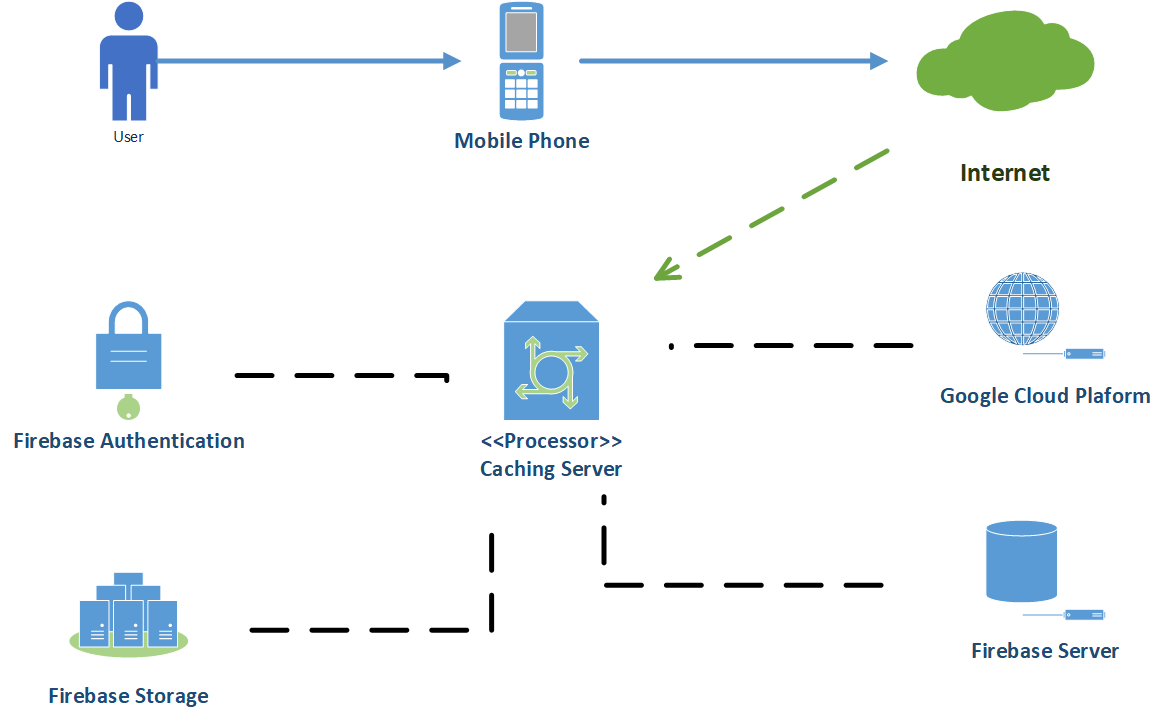
\includegraphics[width=15cm,height=20cm,keepaspectratio]{DeploymentDiagram}
\caption{Deployment Diagram}
\label{fig:Deployment Diagram}
\end{figure}

\begin{figure}

\subsection{Module} 
I don’t know what to write here
\end{figure}
\begin{figure}

\subsection{Security} 		

 I don’t know what to write here
\end{figure}

\begin{figure}

\section{Low Level Design} 
\center
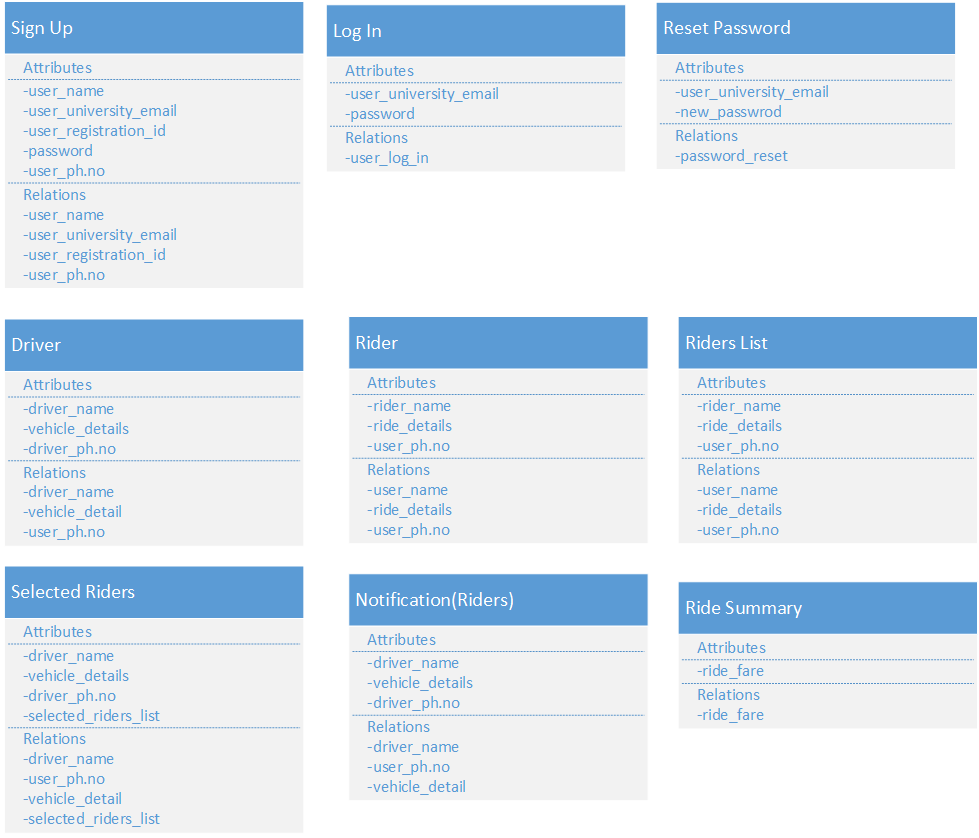
\includegraphics[width=16cm,height=25cm,keepaspectratio]{LowLevelDesign}
\caption{Low Level Design}
\label{fig:Low Level Design}
\end{figure}

\begin{figure}
\section{Database Design}
Firebase platform provides a cloud-hosted Realtime Database. It is a NoSQL cloud database. Data synchronizes among all clients and stays available even when the app goes offline. As it is a NoSQL database, so its functionality is different as compared to a relational database. The data is stored in the form of collections and documents. There is no relationship between classes, so there won’t be any schema of our database. Data gets stored as JSON objects. It is more like a cloud-hosted JSON tree. When a person adds data to the JSON tree, it becomes a node in the existing JSON structure with an associated key. The best method is to use the denormalization technique; using which we split data into separate paths. It becomes easier to download the data in separate calls as required.
\end{figure}

\begin{figure}
\section{GUI Design}
Our application contains more than fifteen screens, different screens based on user type are:
\end{figure}



\begin{figure}
\subsection{Login and Signup Screens}
\hspace*{\fill}
\subfloat[Welcome Screen]{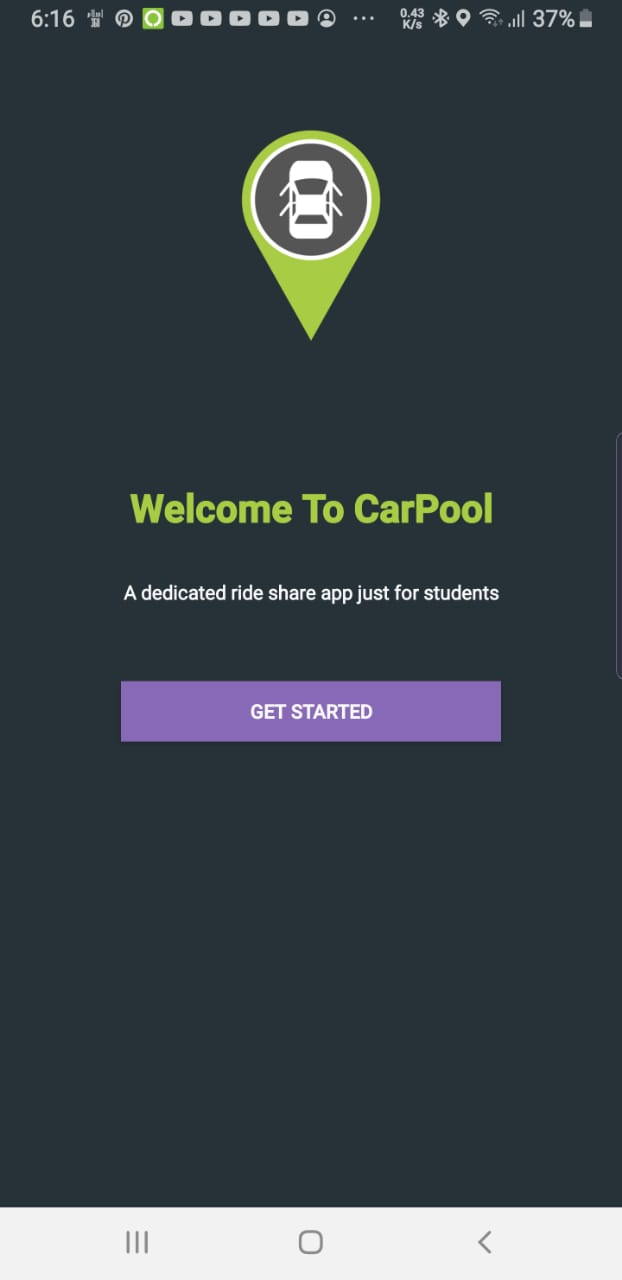
\includegraphics[width = 2in]{S1}}\hfill 
\subfloat[Login Screen]{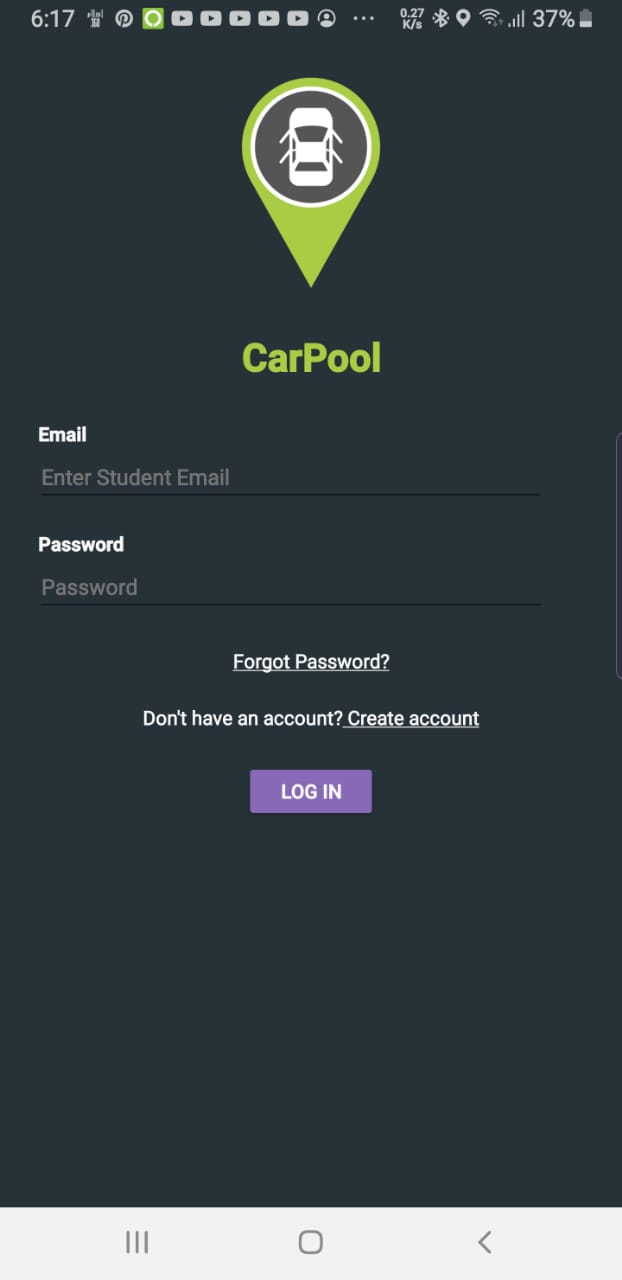
\includegraphics[width = 2in]{S2}}
\hspace*{\fill}

\end{figure}

\begin{figure}
\hspace*{\fill}
\subfloat[Signup Screen]{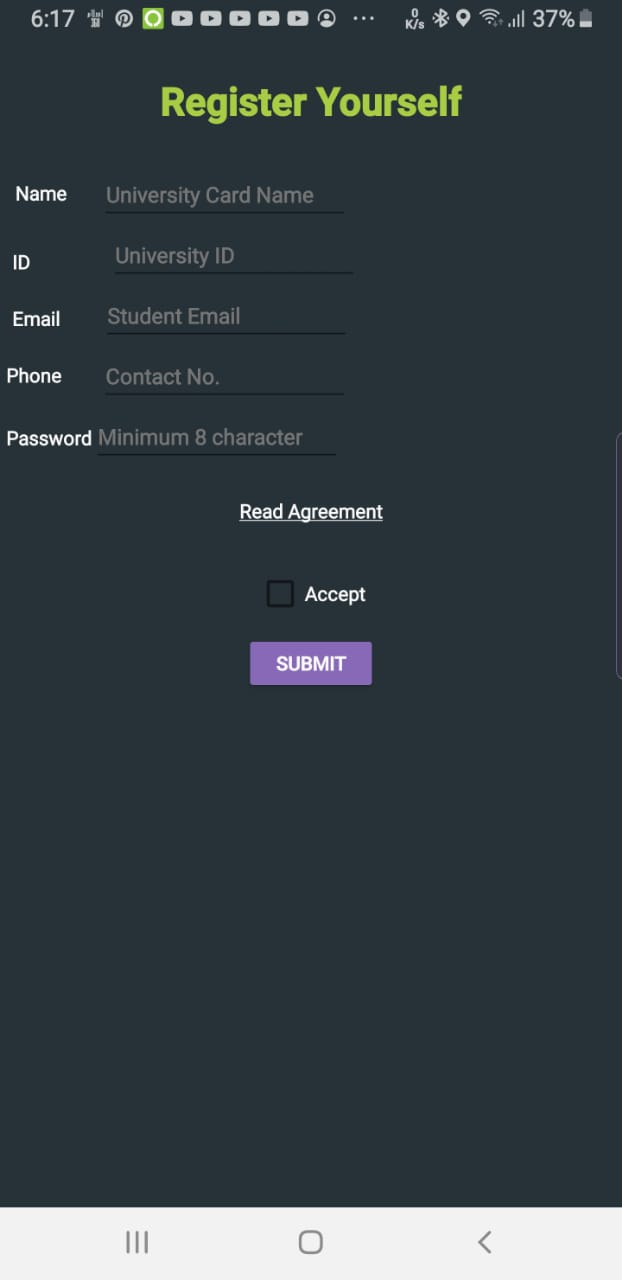
\includegraphics[width = 2in]{S3}}\hfill 
\subfloat[Forgot Password Screen]{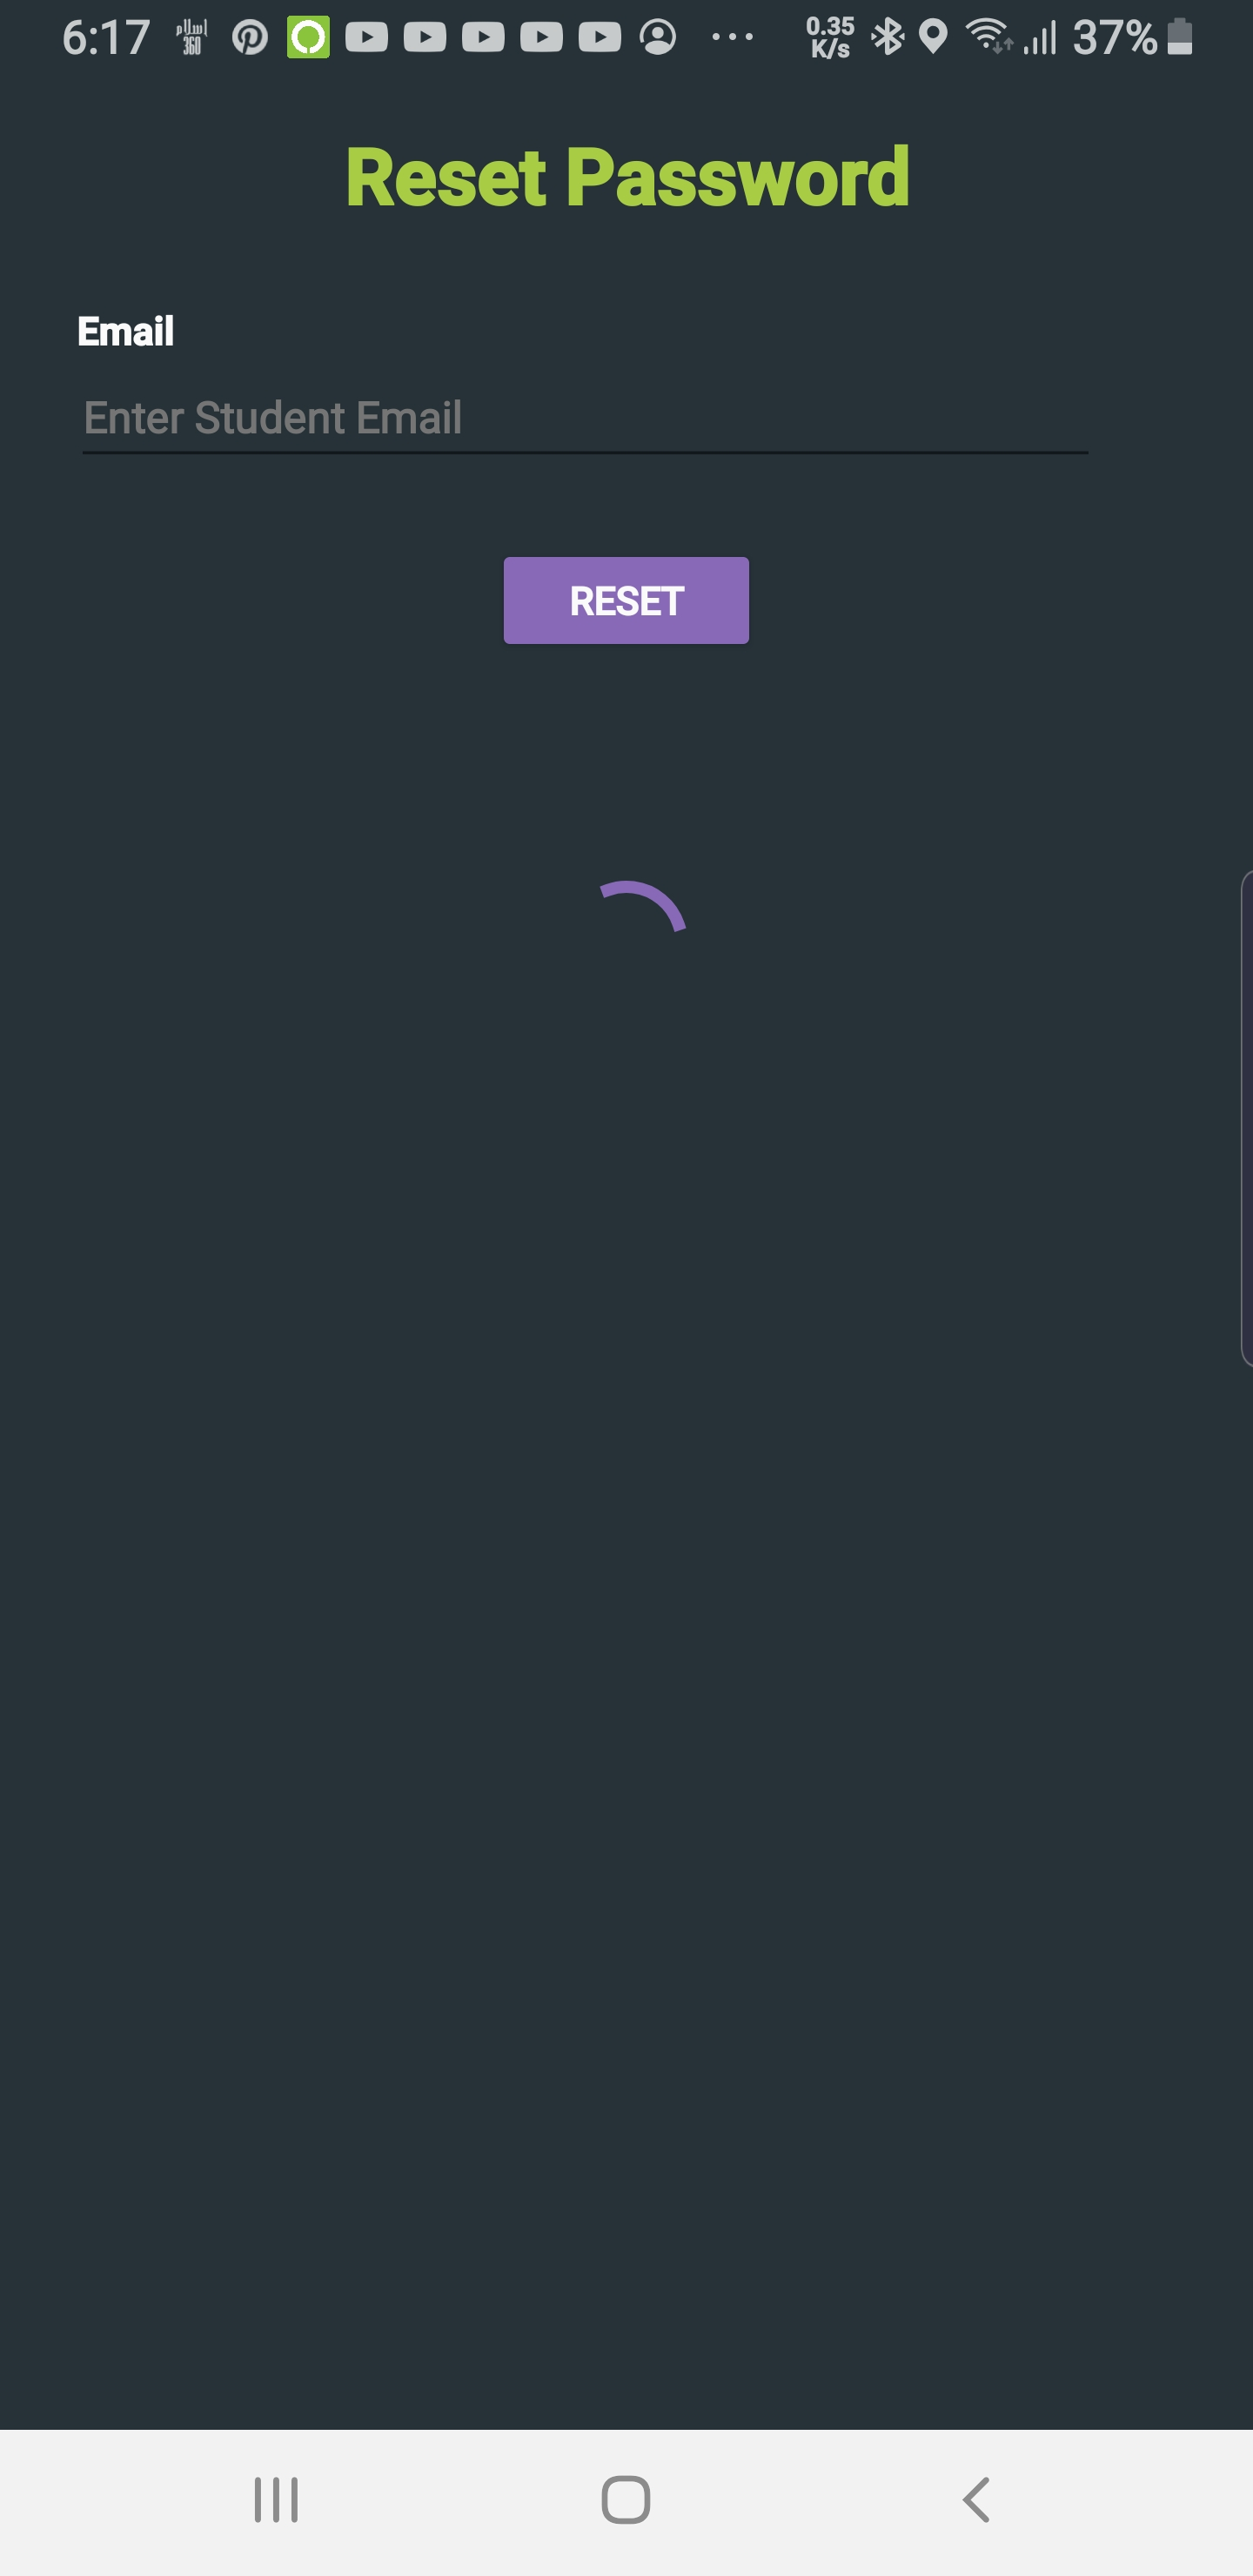
\includegraphics[width = 2in]{S4}}
\hspace*{\fill}
\end{figure}

\begin{figure}
\centering
\subfloat[Select User Type Screen]{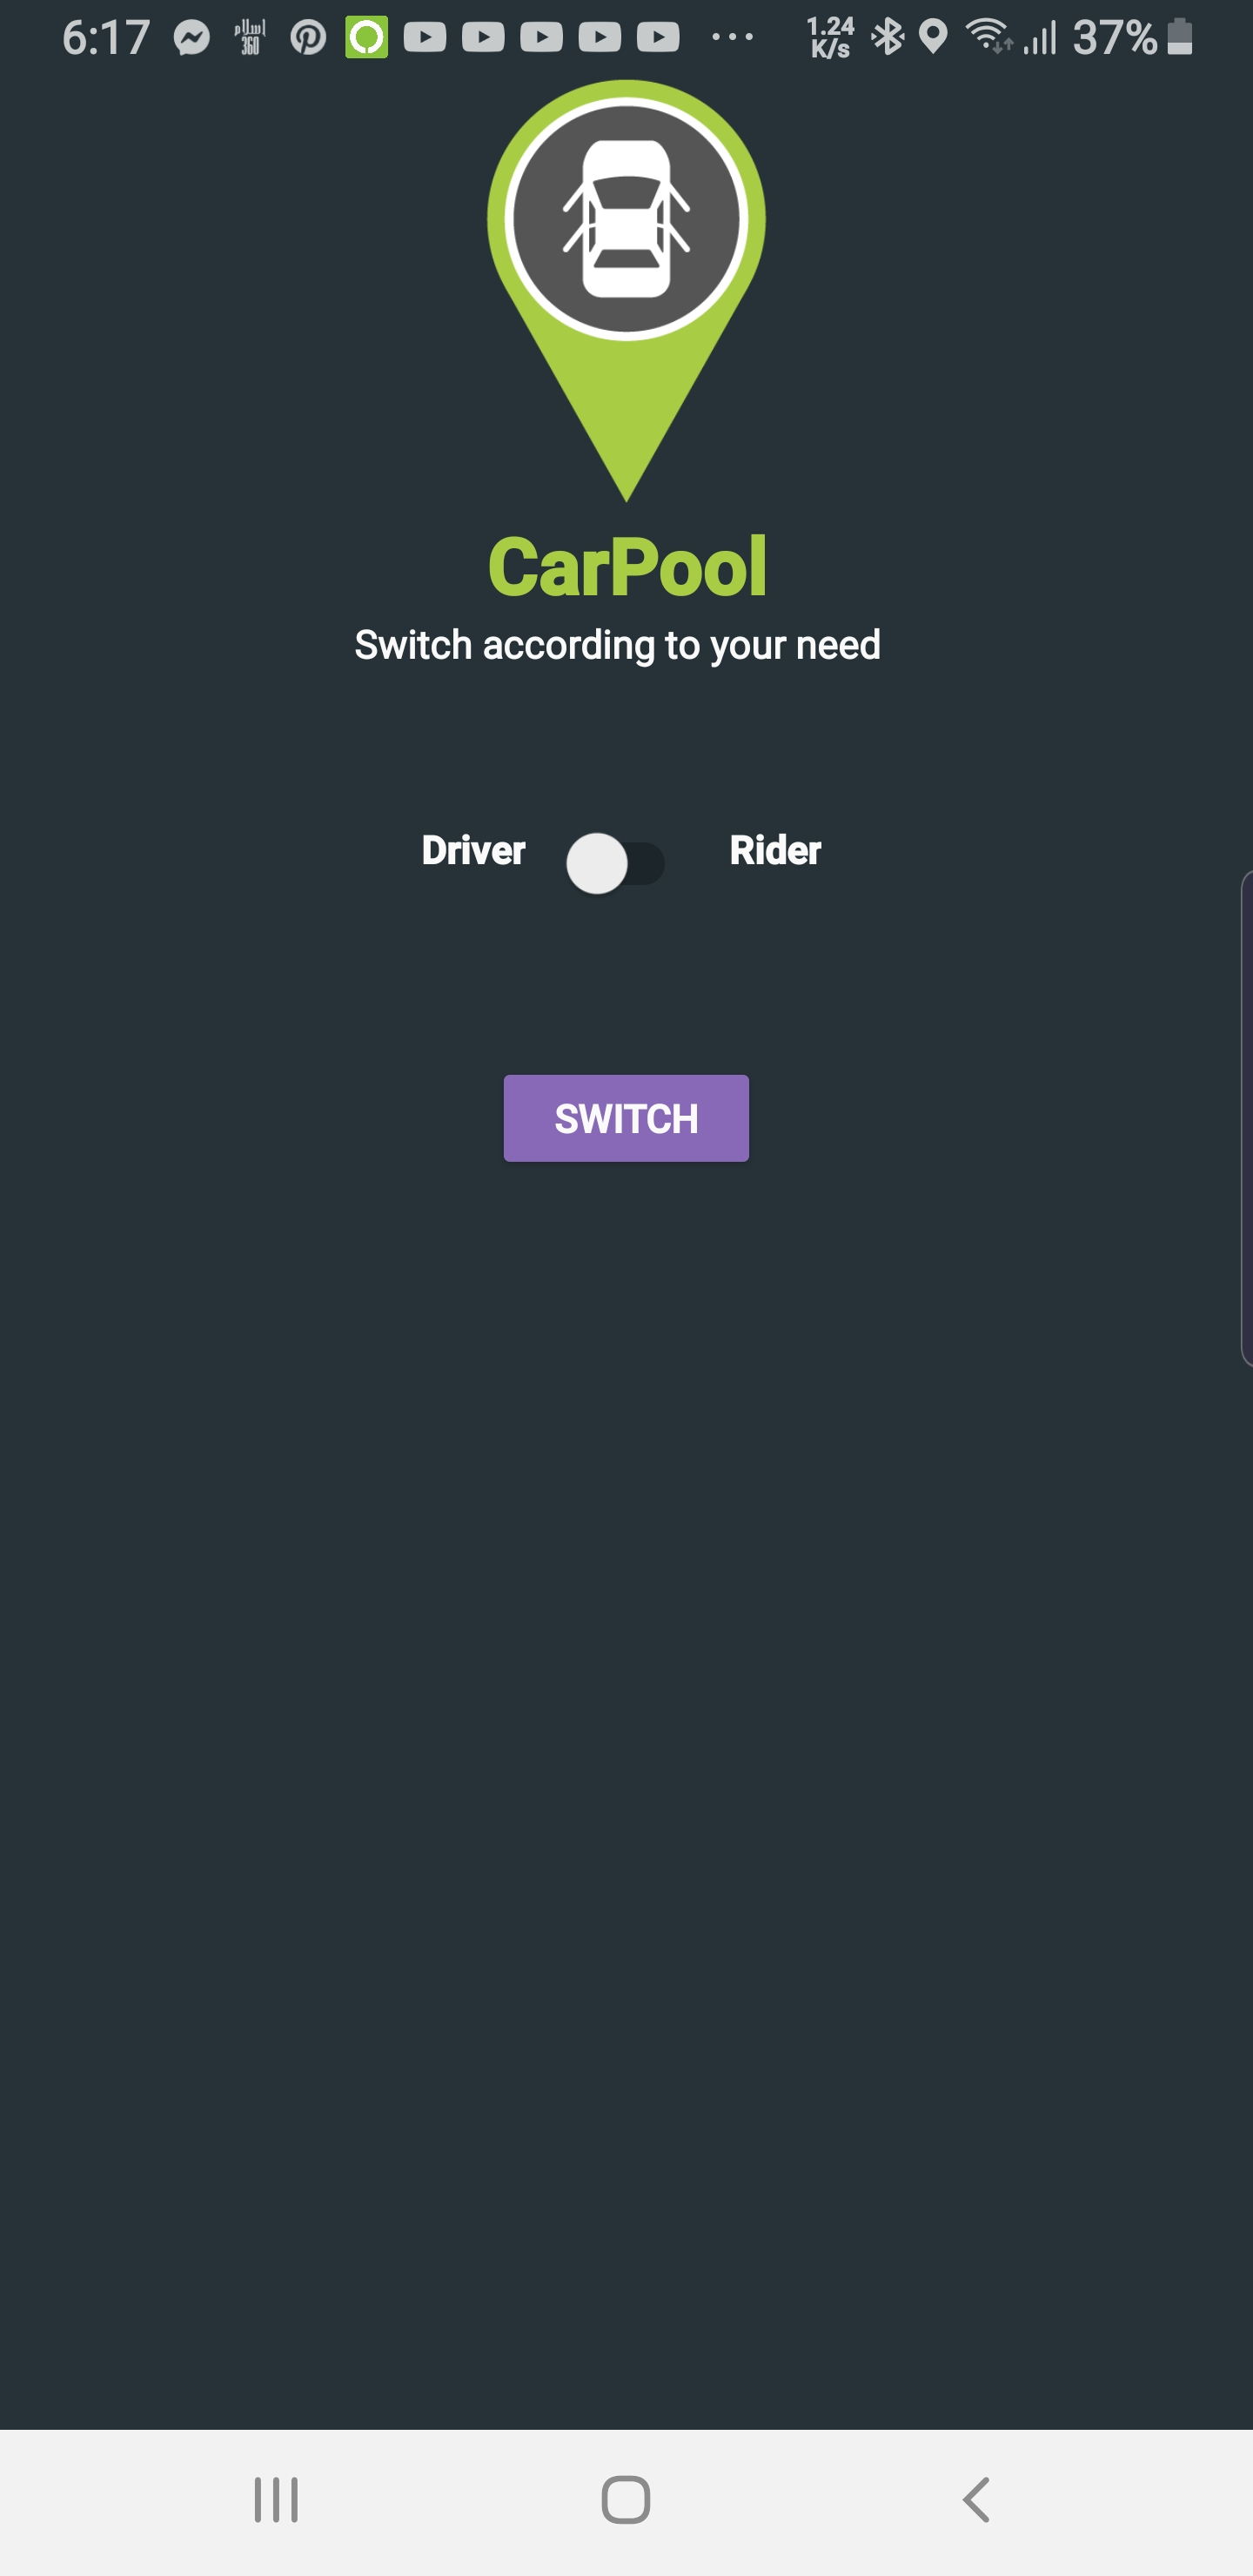
\includegraphics[width = 2in]{S5}}
\end{figure}

\begin{figure}
\subsubsection{Rider Screens}
\hspace*{\fill}
\subfloat[Enter Ride Detail Screen]{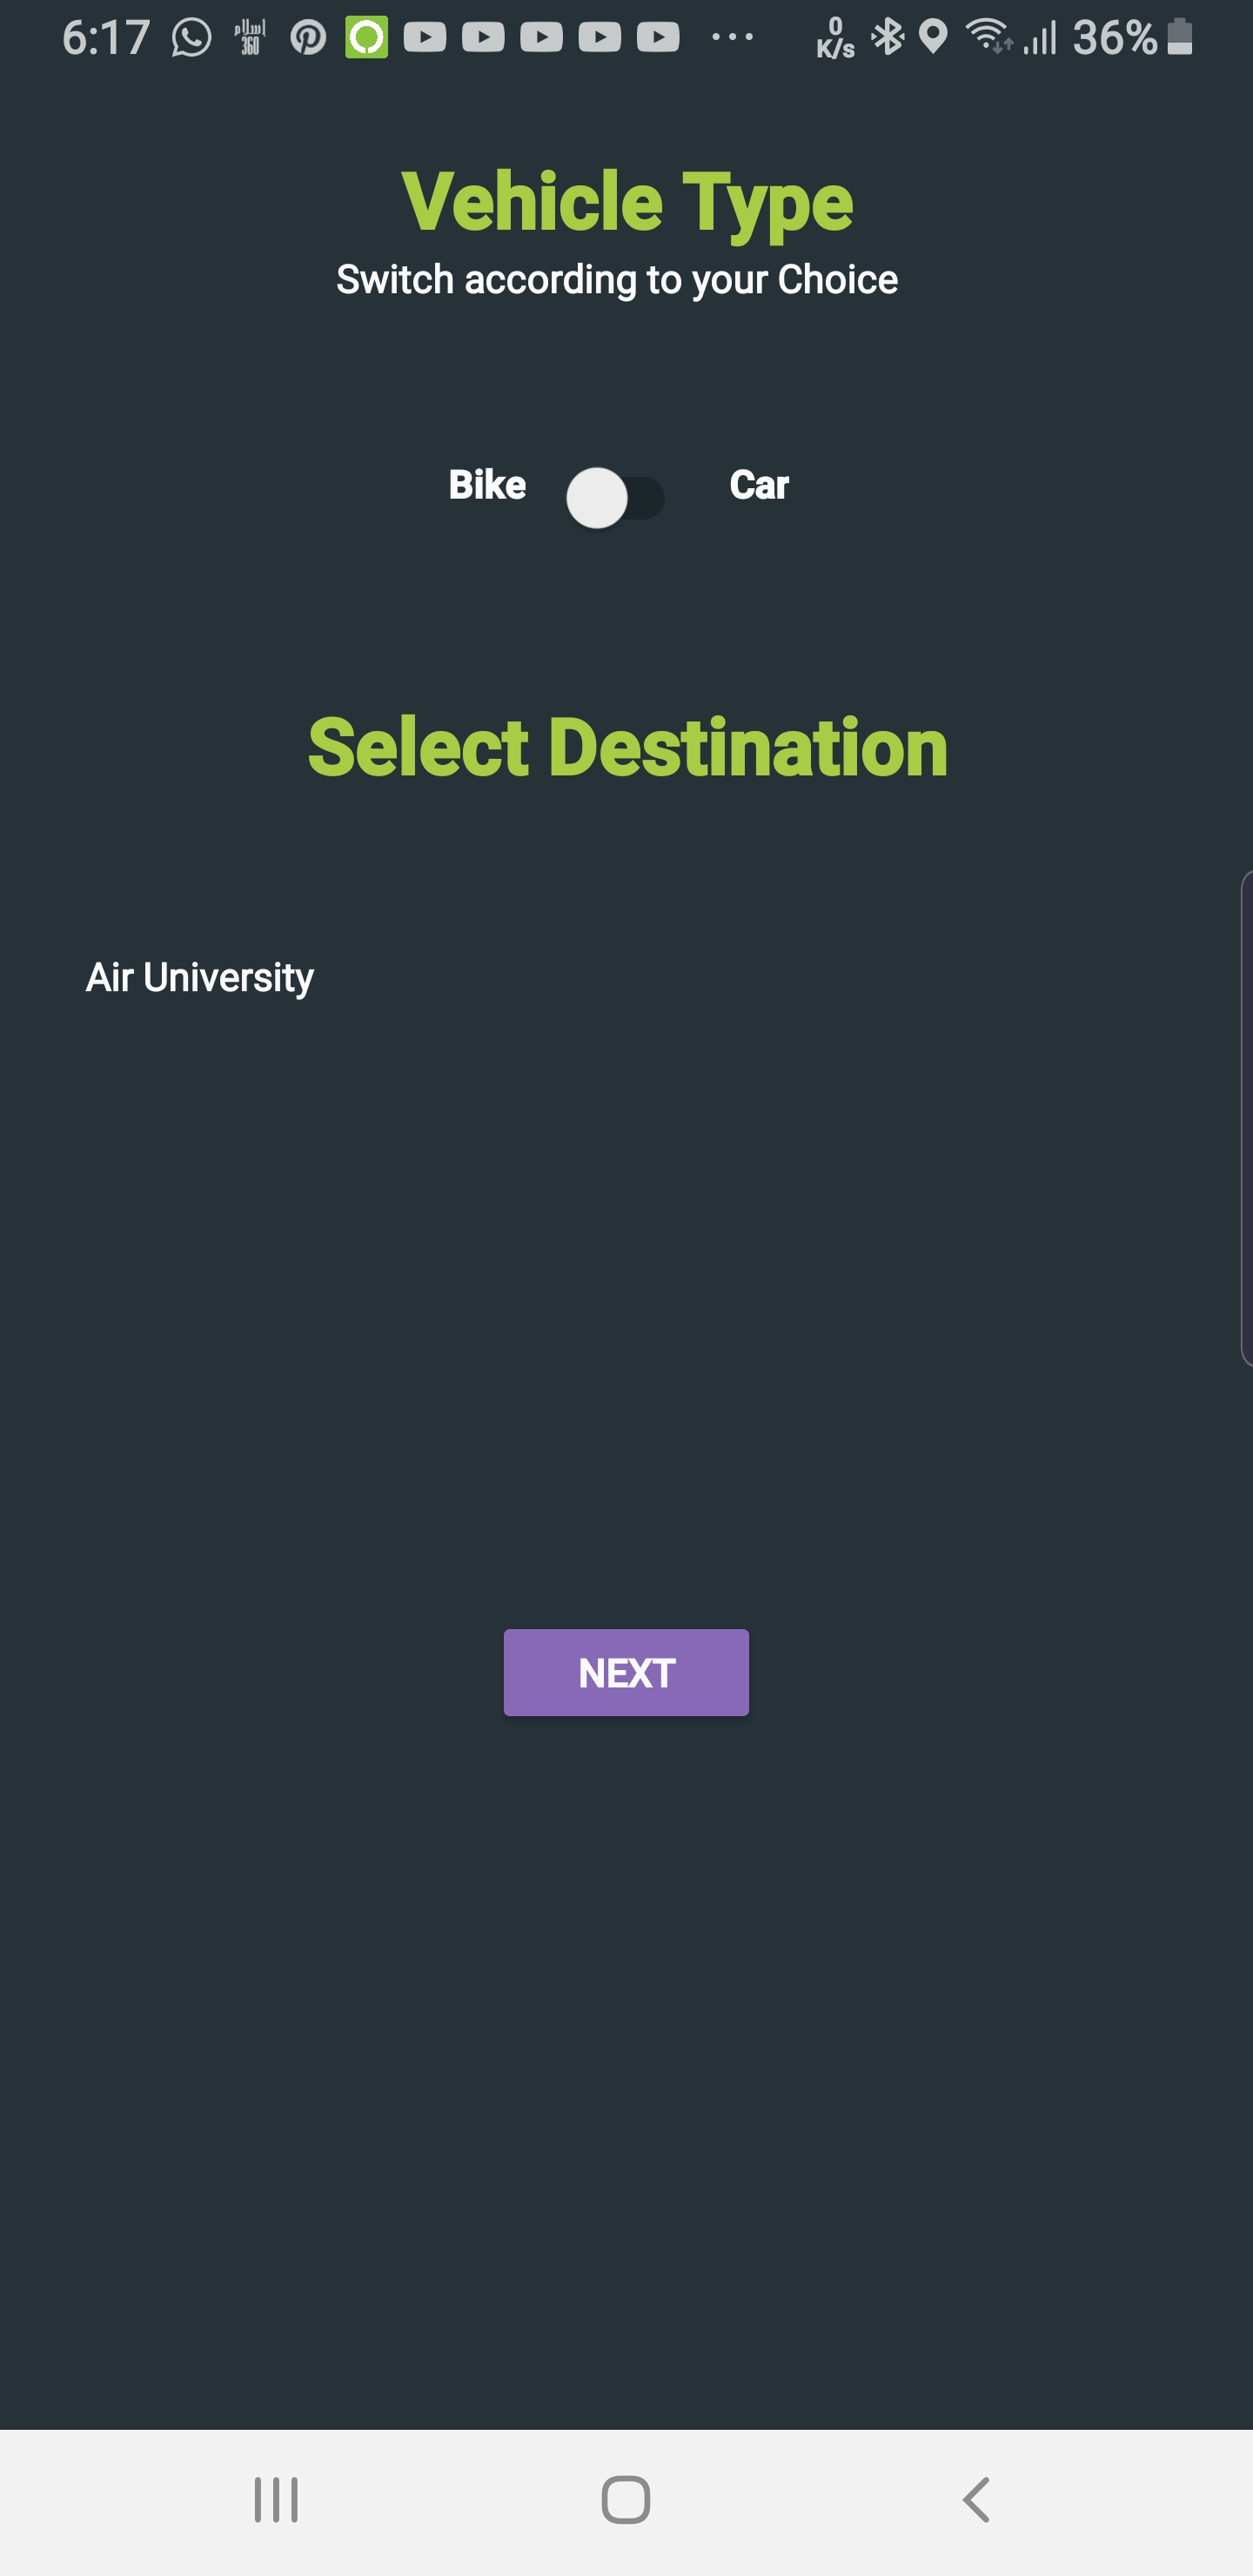
\includegraphics[width = 2in]{S6}}\hfill 
\subfloat[Map Screen]{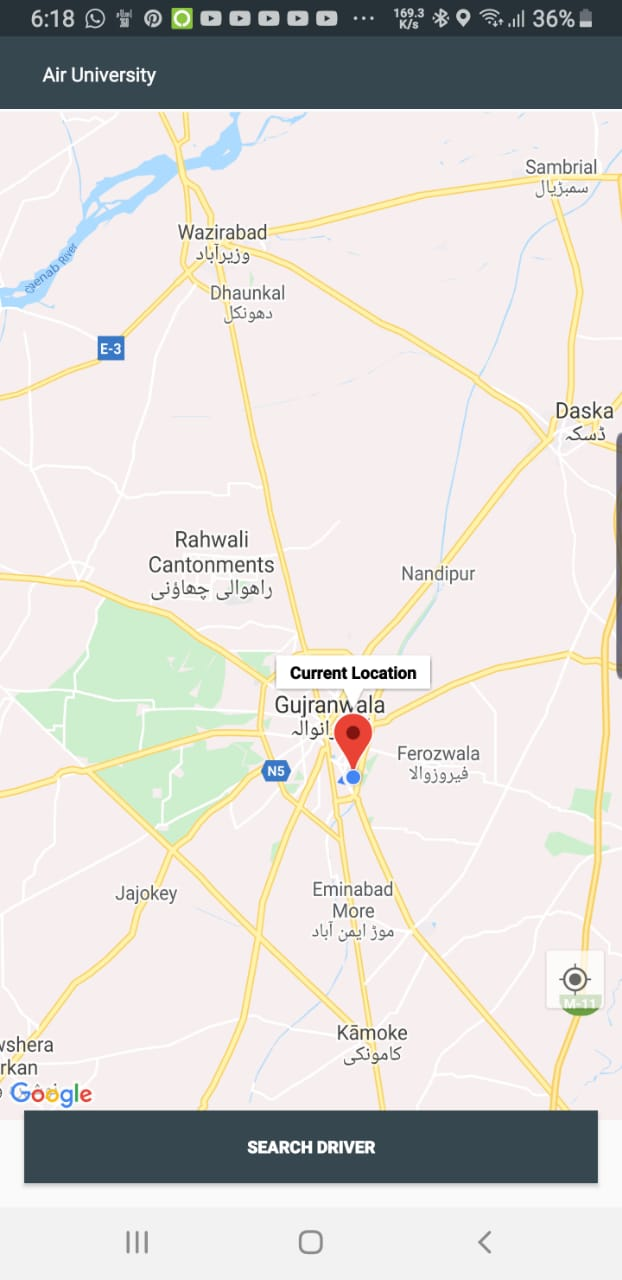
\includegraphics[width = 2in]{S7}}
\hspace*{\fill}\\
\hspace*{\fill}
\subfloat[Driver Detail Screen]{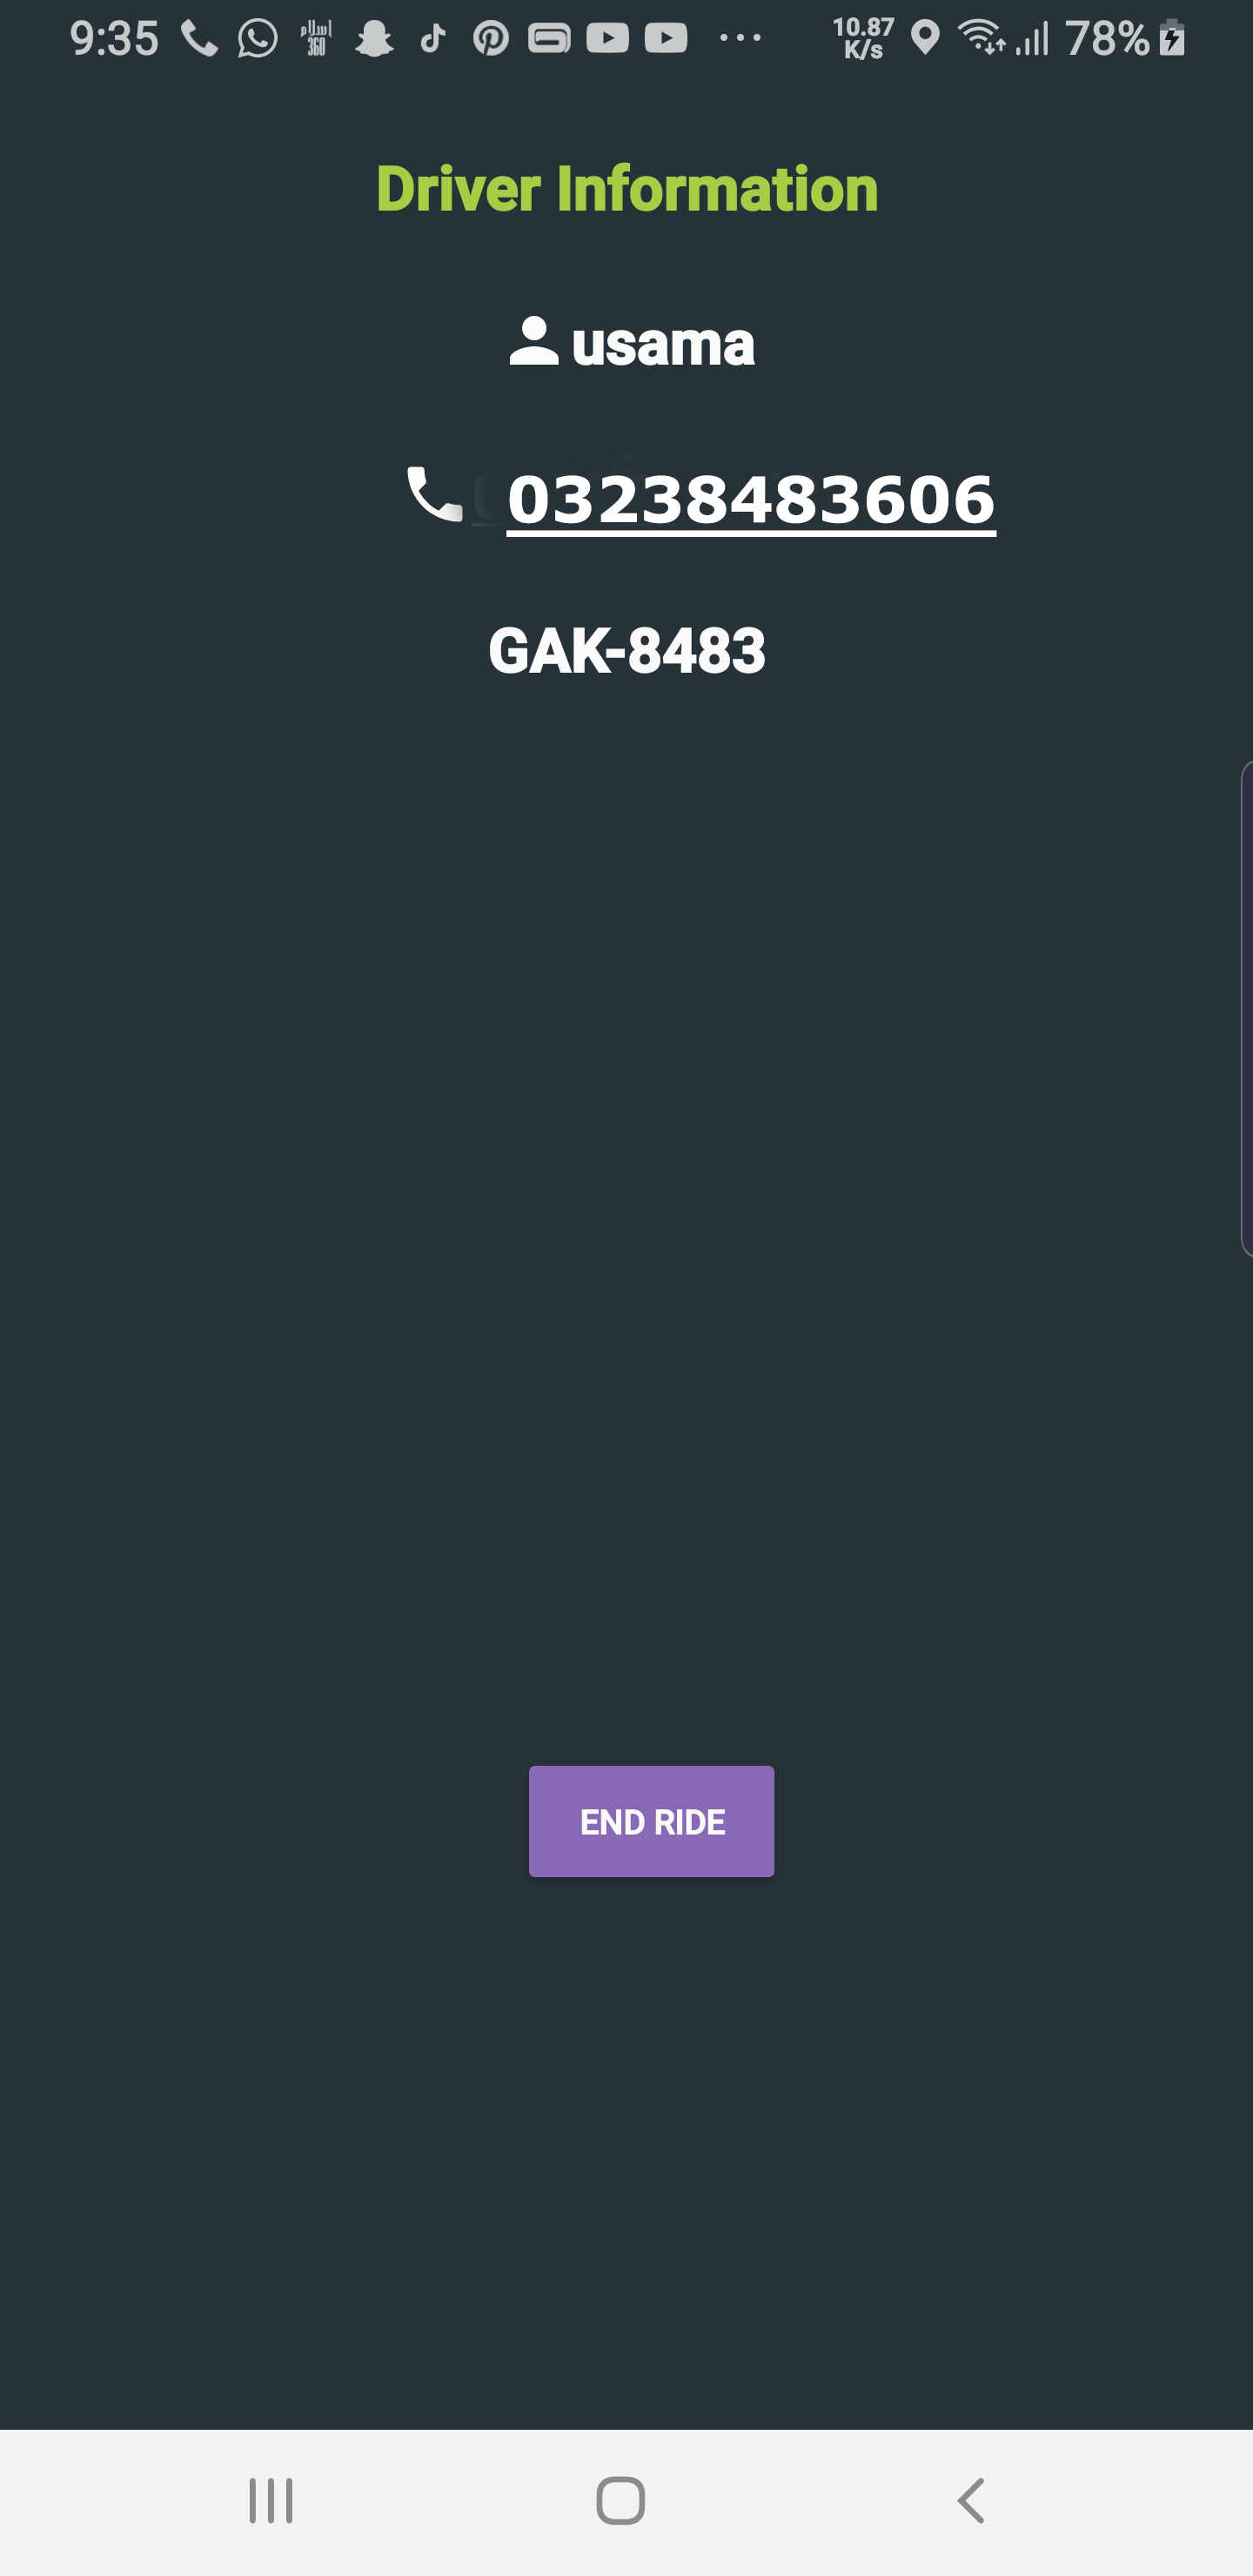
\includegraphics[width = 2in]{S8}}\hfill 
\subfloat[Ride Summary Screen]{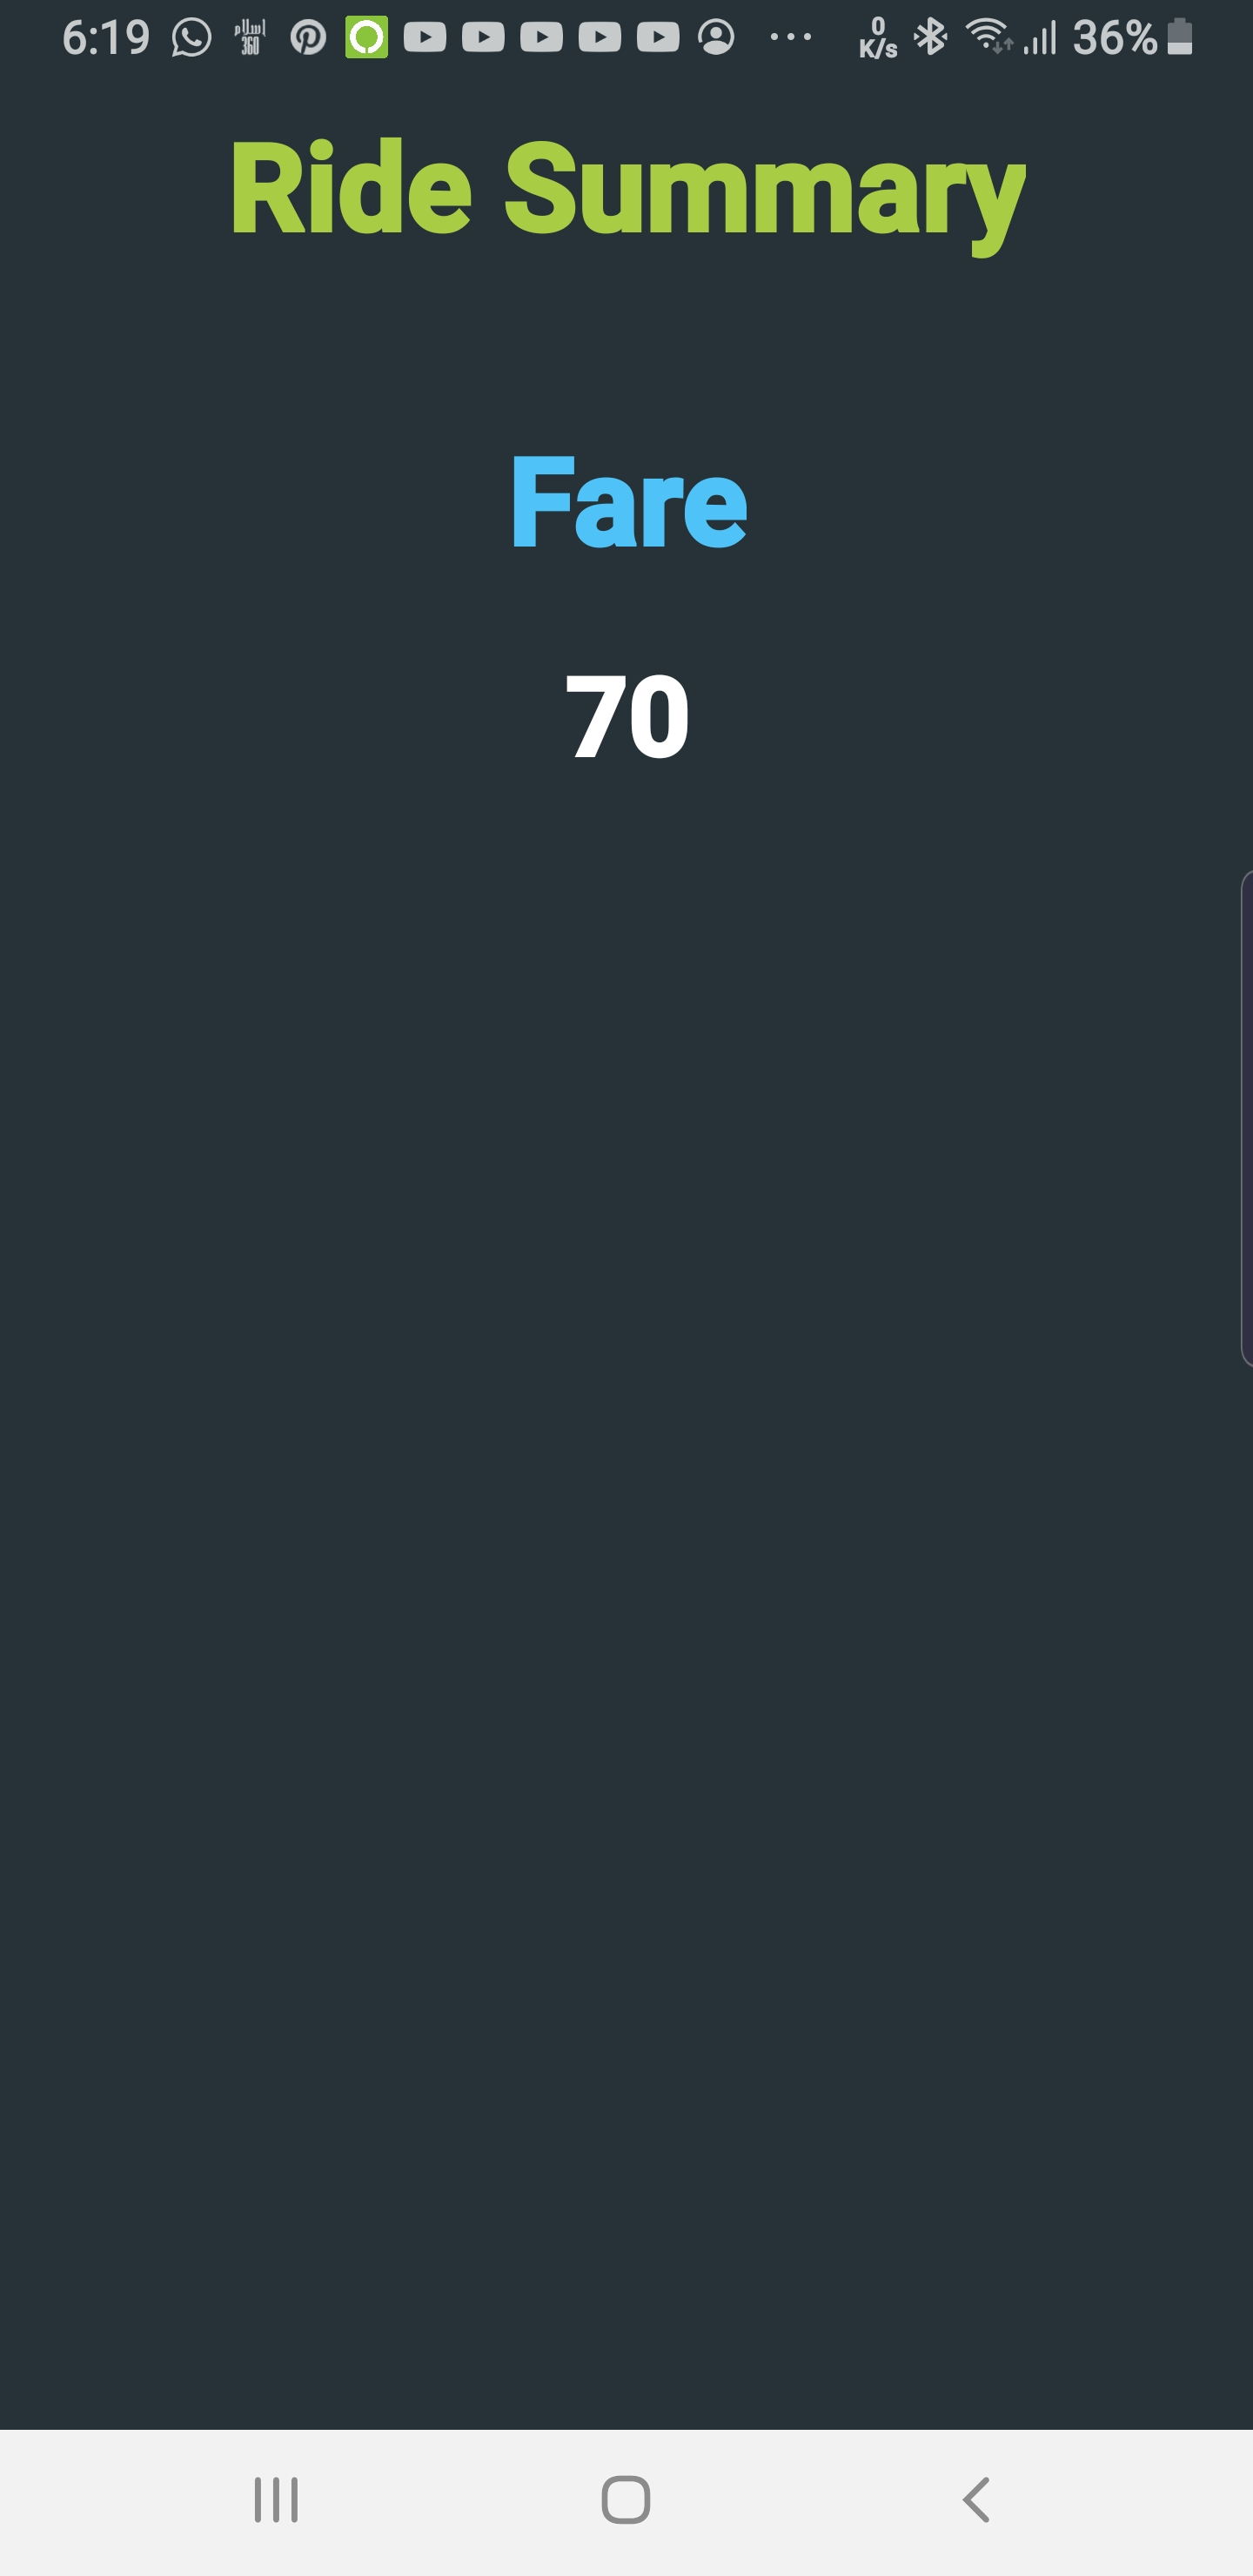
\includegraphics[width = 2in]{S9}}
\hspace*{\fill}
\end{figure}

\begin{figure}
\subsubsection{Driver Screens}
\hspace*{\fill}
\subfloat[Enter Vehicle Detail Screen]{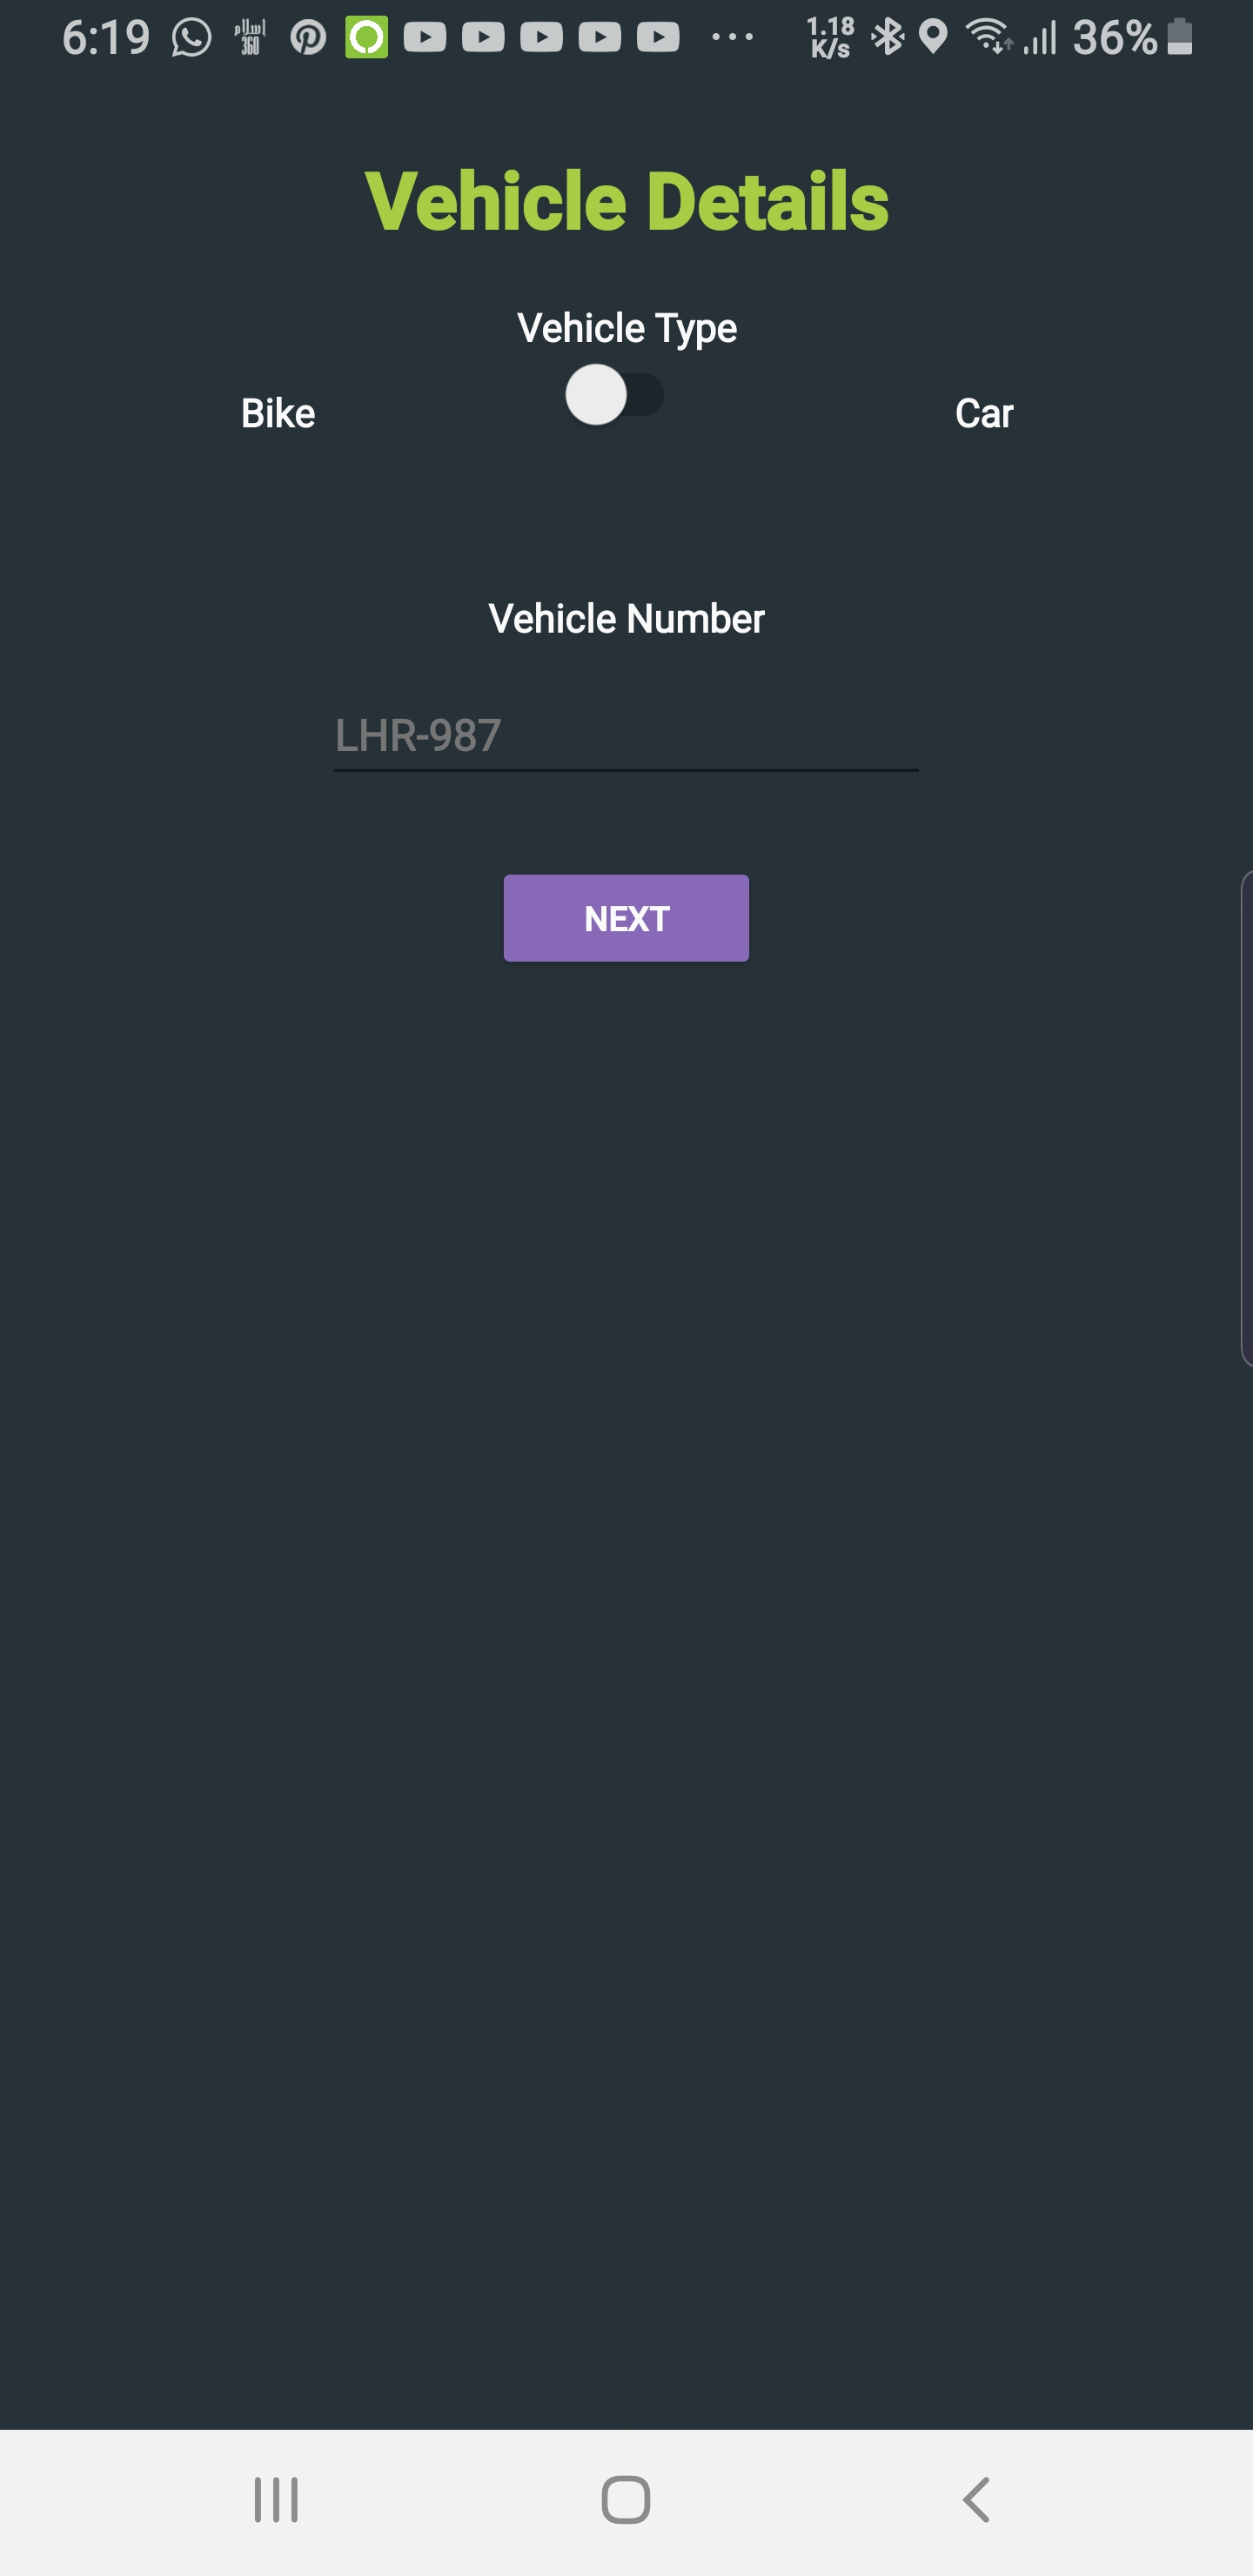
\includegraphics[width = 2in]{S10}}\hfill 
\subfloat[Driver Map Screen]{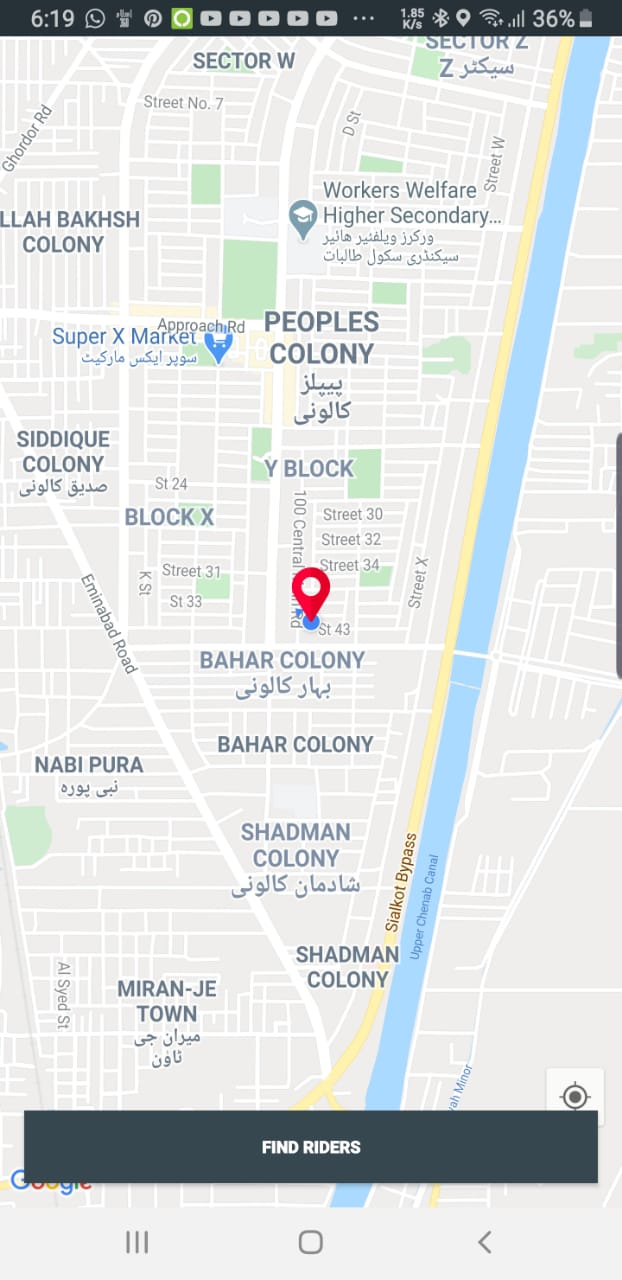
\includegraphics[width = 2in]{S11}}
\hspace*{\fill}\\
\hspace*{\fill}
\subfloat[Rider List Screen]{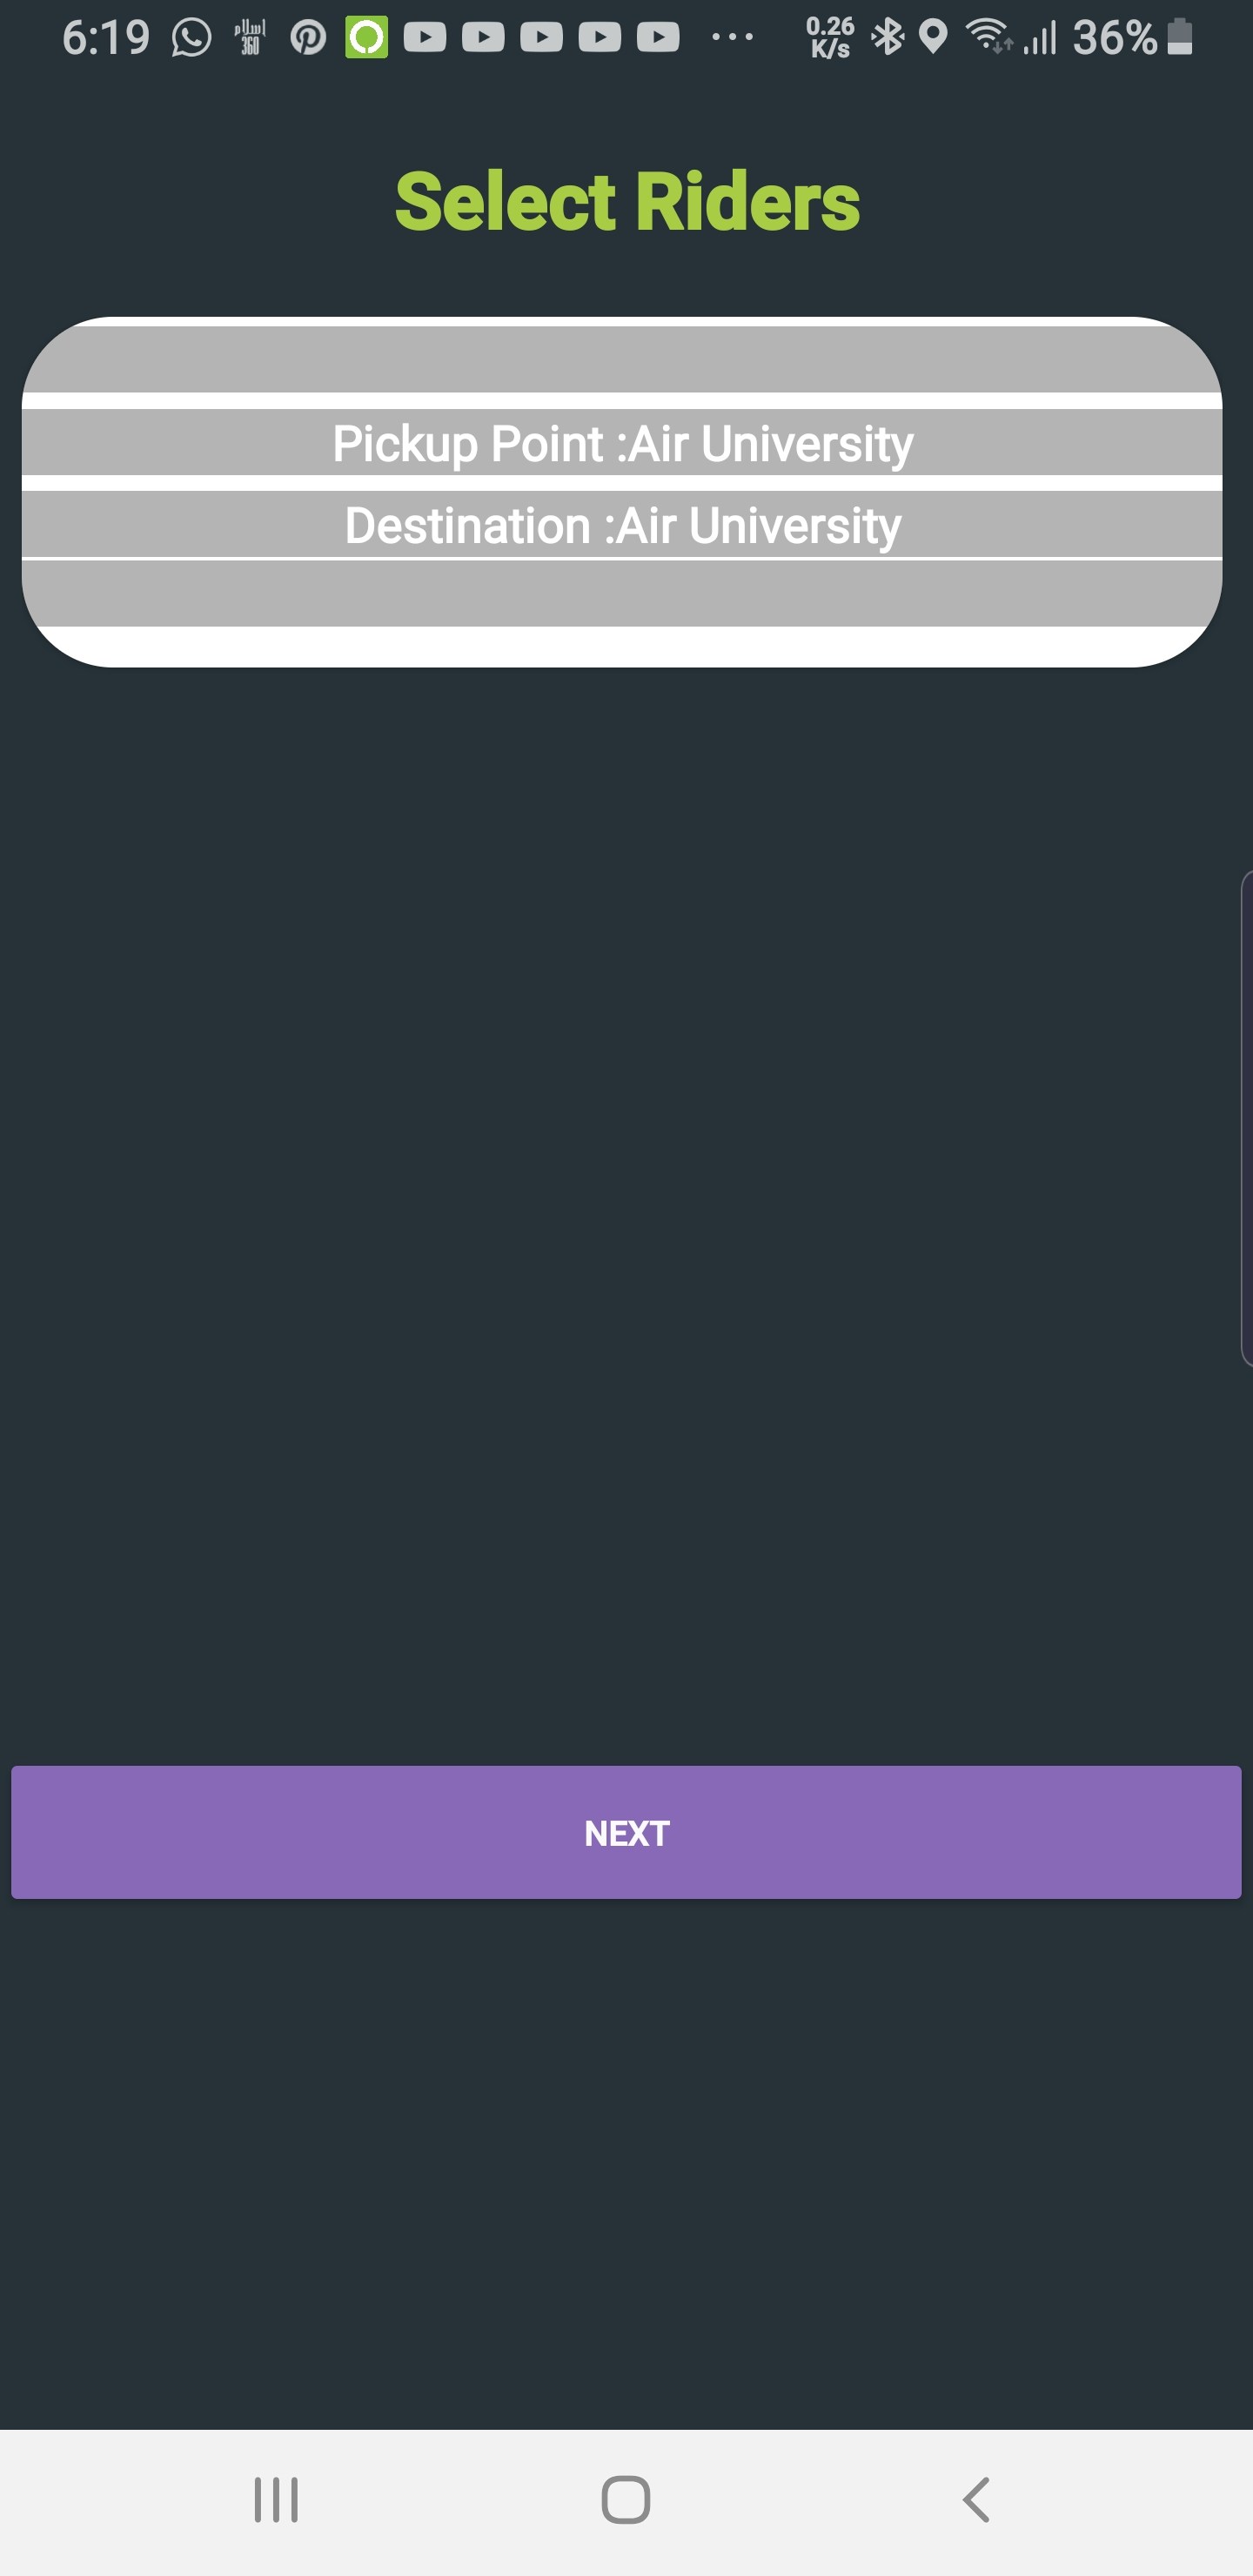
\includegraphics[width = 2in]{S12}}\hfill 
\subfloat[Popup Selection Confirmation Screen]{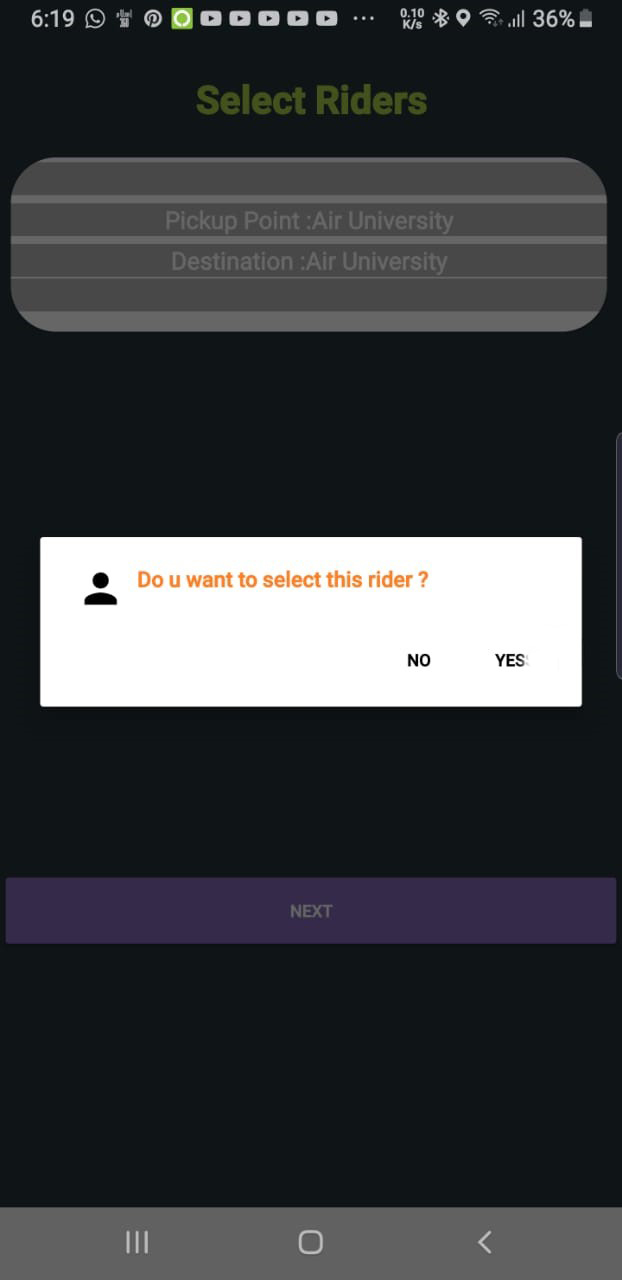
\includegraphics[width = 2in]{S13}}
\hspace*{\fill}
\end{figure}

\begin{figure}
\hspace*{\fill}
\subfloat[Selected Passengers Screen]{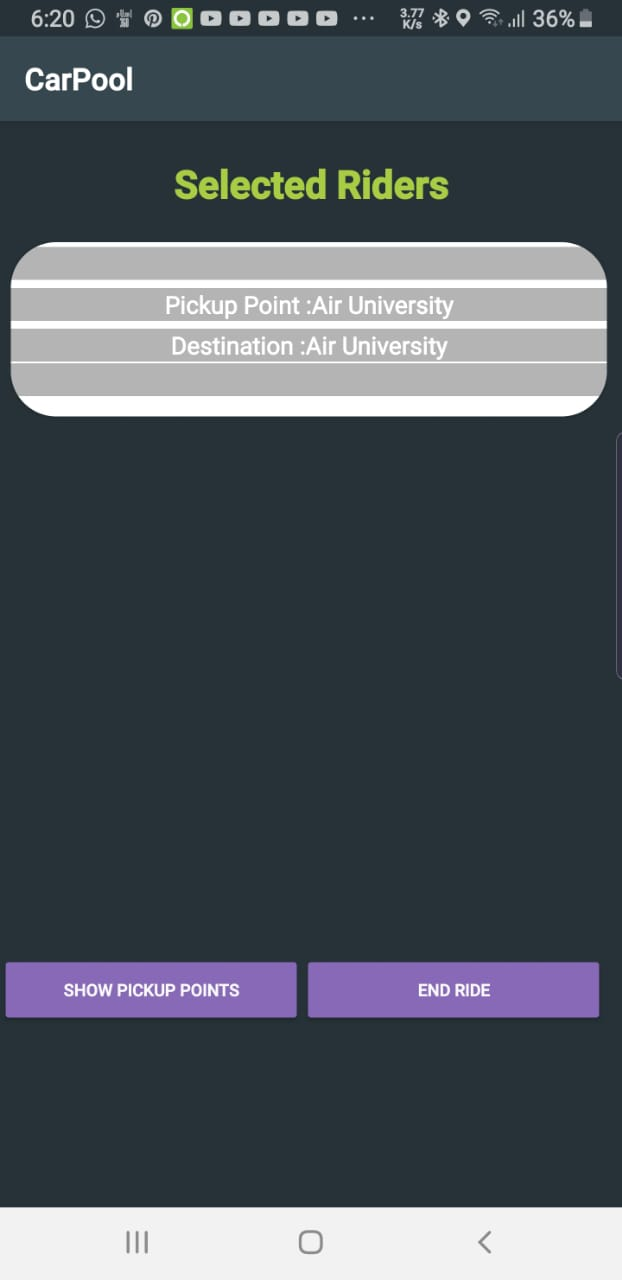
\includegraphics[width = 2in]{S14}}\hfill 
\subfloat[Passengers Pickup Points Screen]{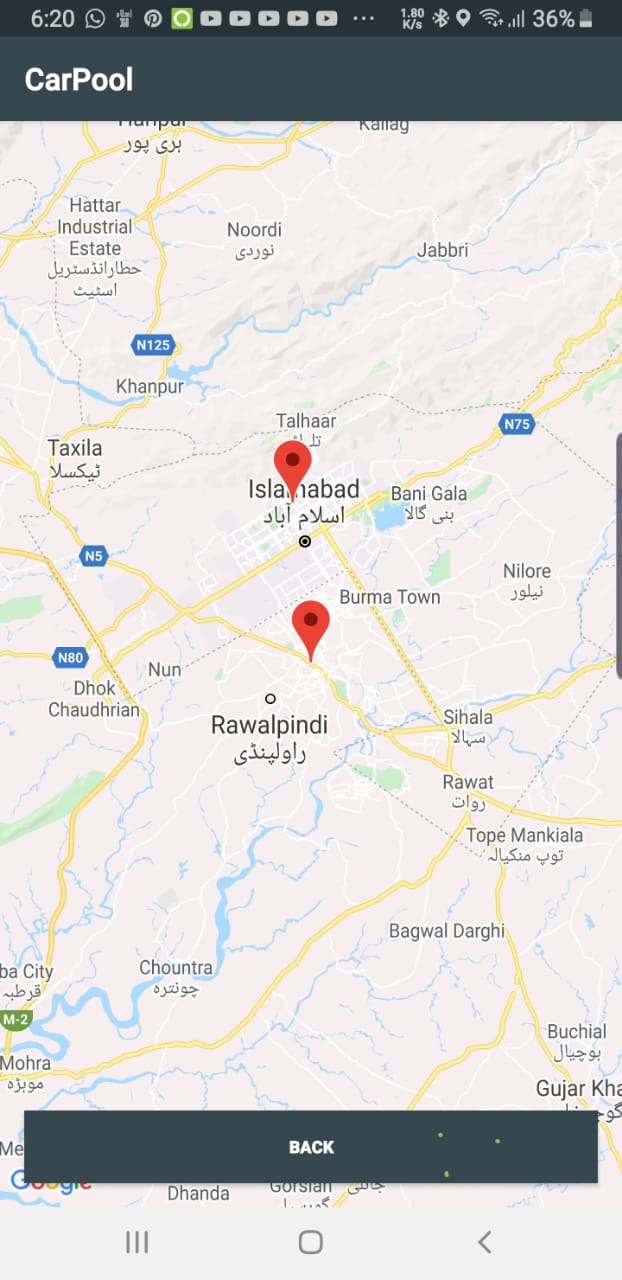
\includegraphics[width = 2in]{S15}}
\hspace*{\fill}
\end{figure}

\begin{figure}
\centering
\subfloat[Driver Summary Screen]{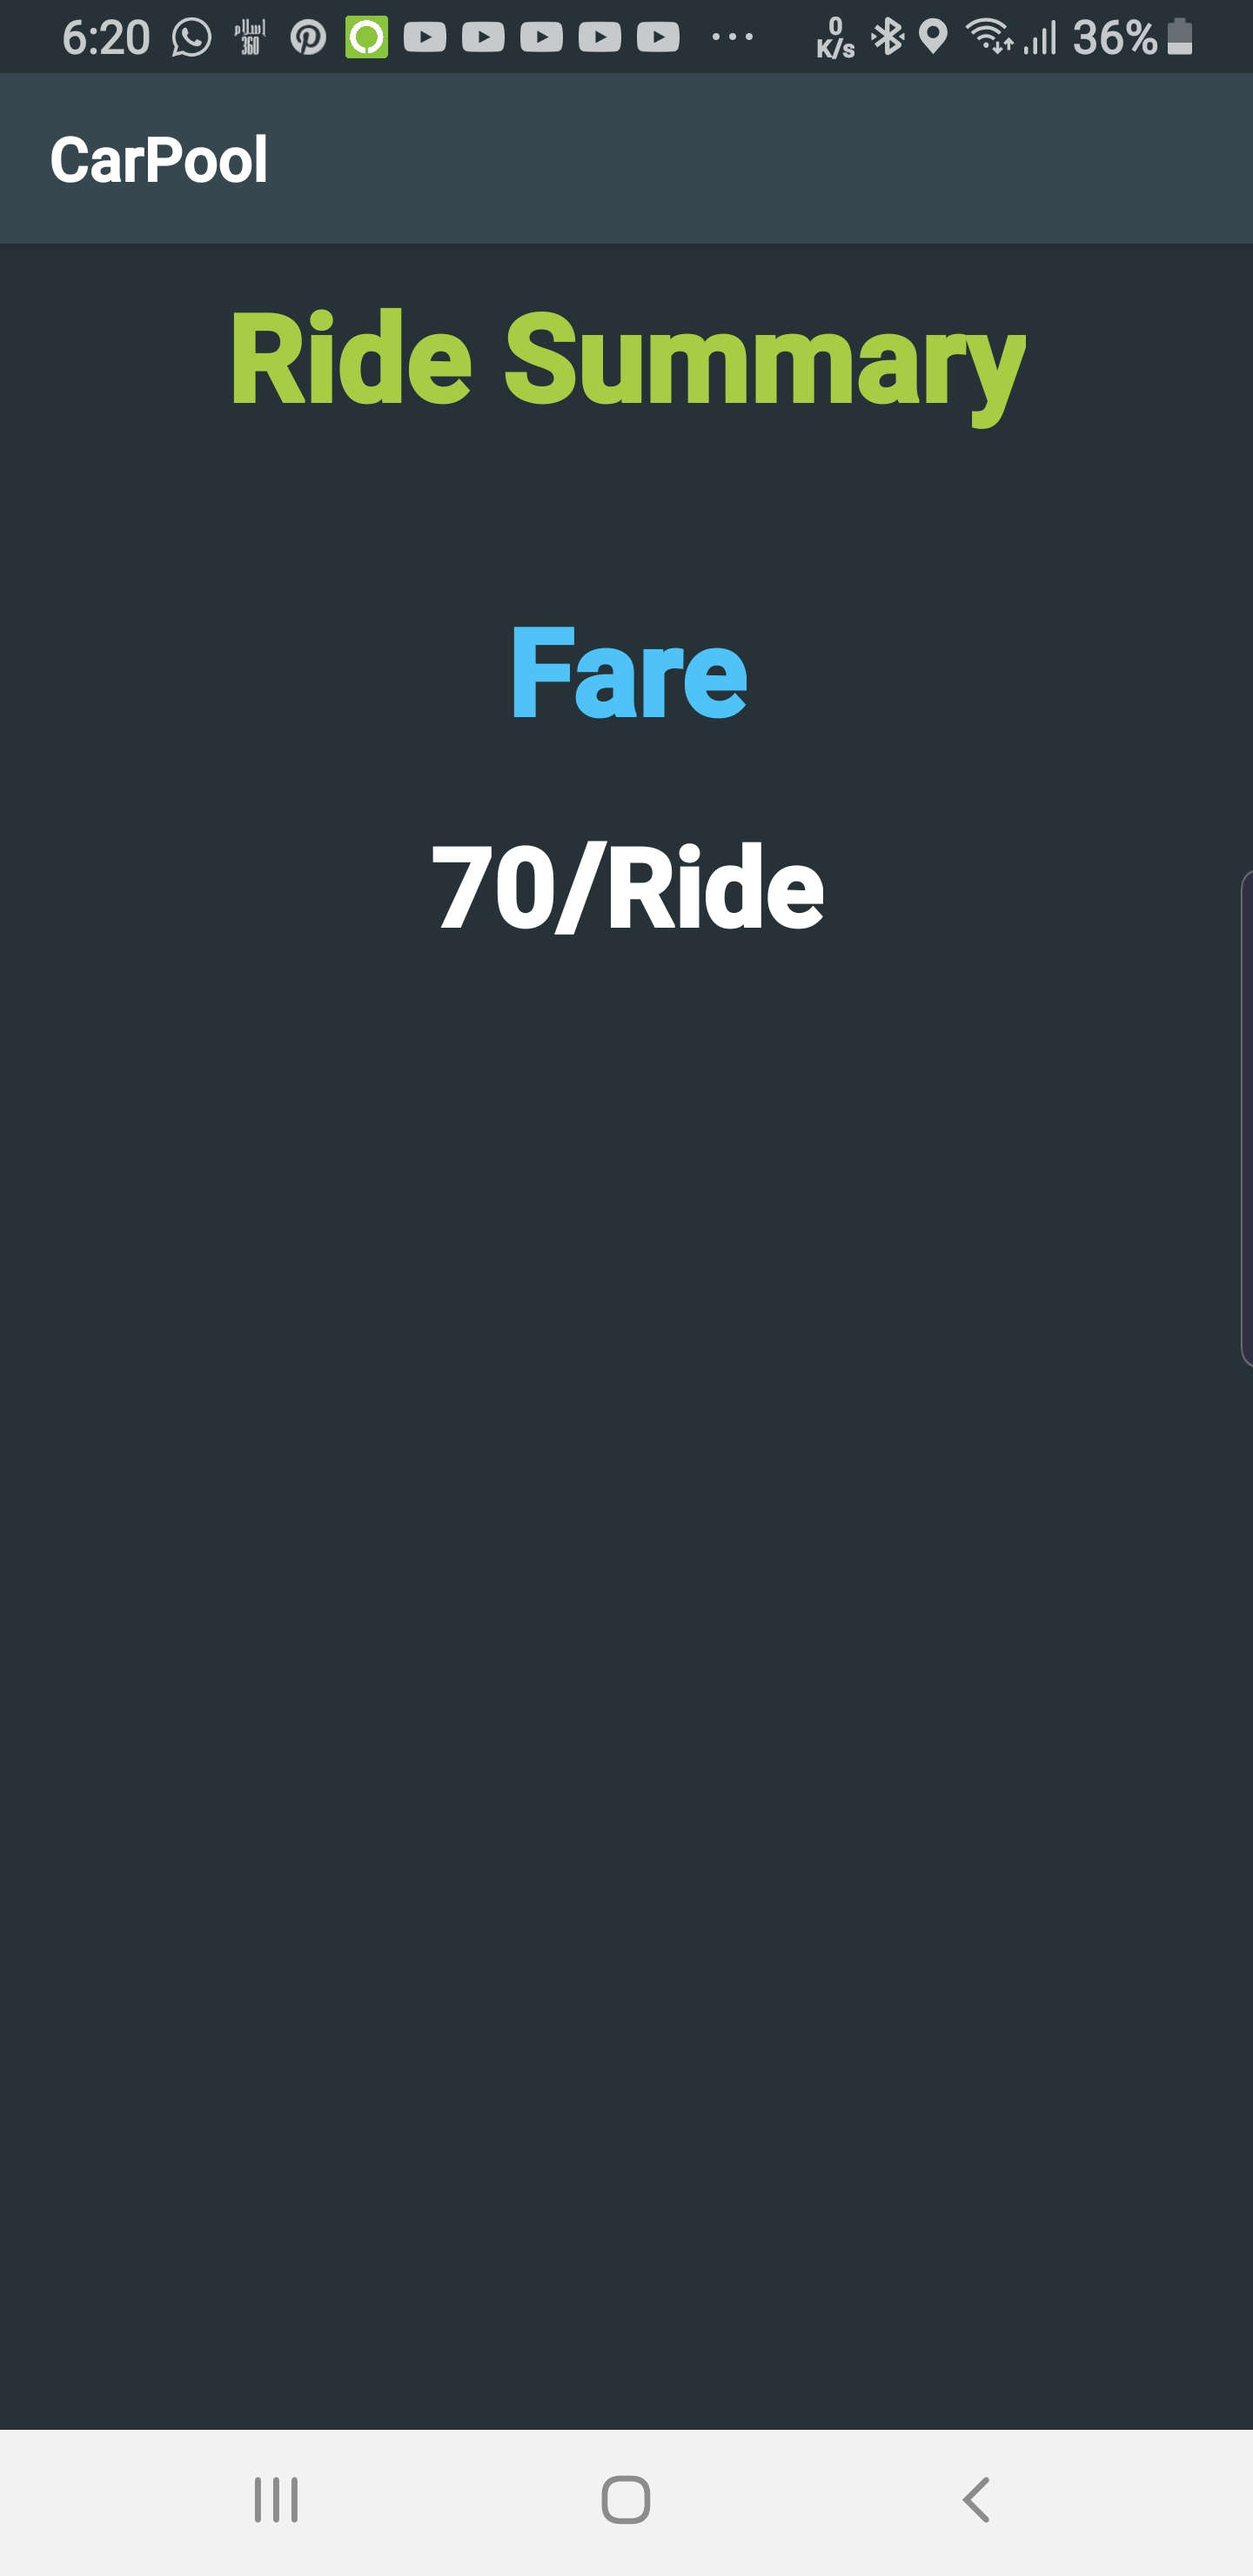
\includegraphics[width = 2in]{S16}}
\end{figure}